\documentclass[11pt]{report}
\textwidth 15.2cm %6.0in  %468pt
\textheight 22.0cm %9.0in  %648pt
%\headheight = 0.0cm
%\headsep = 0.0cm
%\topmargin = 0.0cm
%\footheight = 0.0cm
\footskip = 1.0cm
\baselineskip=4ex


\def\setspacing#1{\renewcommand{\baselinestretch}{2}}

\usepackage{latexsym}
\usepackage{amsmath,amsthm,amssymb,tabularx}
\usepackage{tabularx}
\usepackage{calc}
\usepackage{xspace}
\usepackage{afterpage}
\usepackage{algorithm}
\usepackage{algorithmic}
\usepackage{float}
\usepackage{caption}
\usepackage{setspace}
\usepackage{multirow}
\usepackage{rotating}
\usepackage{cuthesis}
\usepackage{ccaption}
\usepackage{lscape}
\usepackage{amsfonts}
\usepackage{url}
\usepackage{graphicx,subfigure}
\usepackage[latin1]{inputenc}
\usepackage{xspace}
\usepackage{footnote}
\pagestyle{plain}
\usepackage{acronym}
\usepackage{epsfig}
\usepackage{amsfonts}
%\usepackage{array, colortbl}
%%========================================================================
% Omar packages

\usepackage{graphics}
% or use the graphicx package for more complicated commands
 \usepackage{graphicx}
% or use the epsfig package if you prefer to use the old commands
 \usepackage{epsfig}
 \usepackage{epstopdf}
% The amssymb package provides various useful mathematical symbols
\usepackage{amssymb}
%\usepackage[cmex10]{amsmath}
\usepackage{dsfont}
\usepackage{verbatim}
\usepackage{algorithm}
\usepackage{algorithmic}
\newtheorem{definition}{Definition}
\newtheorem{corollary}{Corollary}
\newtheorem{proposition}{Proposition}
\newtheorem{observation}{Observation}
\newtheorem{property}{Property}
\newtheorem{theorem}{Theorem}
\newtheorem{lemma}{Lemma}
\newtheorem{proof*}{Proof}%[section*]
\newtheorem{example}{Example}
%%========================================================================
\def\boxit#1{\leavevmode\hbox{\vrule\vtop{\vbox{\kern.33333pt\hrule
   \kern1pt\hbox{\kern1pt\vbox{#1}\kern1pt}}\kern1pt\hrule}\vrule}}
%
% Different font in captions
% Different font in captions
\setlength{\abovecaptionskip}{0pt}   % 0.5cm as an example
%\setlength{\belowcaptionskip}{0pt}   % 0.5cm as an example


\usepackage{amsmath}
\makeatletter
\g@addto@macro\normalsize{%
  \setlength\abovedisplayskip{5pt}
  \setlength\belowdisplayskip{5pt}
  \setlength\abovedisplayshortskip{5pt}
  \setlength\belowdisplayshortskip{5pt}
}

\pagestyle{myheadings}
\setcounter{secnumdepth}{3}
\setcounter{tocdepth}{3}


\normalsize \setlength{\headheight}{\baselineskip}
\setlength{\headsep}{\baselineskip}
\newcommand{\longpage}{\enlargethispage{\baselineskip}} % Latex companion p 99
\makeatletter
\oddsidemargin 0.5in \evensidemargin 0.5in
\marginparwidth 40pt \marginparsep 10pt
%\topmargin 0pt \headsep .5in         % no longer acceptable
%\textheight 8.1in \textwidth 6in     % no longer acceptable
%\topmargin 0in \headsep 0in %-0.1 topmargin
\topmargin -0.2in \headsep 0in %-0.1 topmargin
\textheight 8.75in \textwidth 6in %9in textheight
\brokenpenalty=10000
\renewcommand{\baselinestretch}{1.5}
%%%%%%%%%%%%%%%%%%%%%%%%%%%%%%%%%%%%%%%%%%%%%%%%%%%%%%%%%%%%%%%%%%%%%%added dec 1st


\renewcommand{\contentsname}{Table of Contents}
\parskip \medskipamount
\renewcommand{\captionfont}{\em}

%
% Try to get the code lines as close to the line width as possible.
% (i.e., try to get the lgrind line numbers as close as possible to
% the right margin.)
%
\newlength{\lgrindlinewidth}
\newlength{\lgrindlabelwidth}
\settowidth{\lgrindlabelwidth}{\tiny 0000}
\setlength{\lgrindlinewidth}{\textwidth-\lgrindlabelwidth}
%
% float parameters
%
\renewcommand{\topfraction}{0.90}
\renewcommand{\bottomfraction}{0.90}
\renewcommand{\textfraction}{0.25} % FAQ says 1 - float fraction
\renewcommand{\floatpagefraction}{0.90}

%%%%%%%%%%%%%%%%%%%%%%%%%%%%%%%%%%%%%%%%%%%%%%%%%%%%%%%%%%%%%%%%%%%%%%%
%                        MF abbreviations
%%%%%%%%%%%%%%%%%%%%%%%%%%%%%%%%%%%%%%%%%%%%%%%%%%%%%%%%%%%%%%%%%%%%%
%often used phrases
\newcommand{\bhma}{breath-hold misalignment }
\newcommand{\bhmas}{breath-hold misalignments }
\newcommand{\etal}{\textit{et al. }}
%transform arrow
\newcommand{\TR}{$ {\Rightarrow} $}
\newcommand{\aTR}{$ \stackrel{T_A}{\Rightarrow} $}
\newcommand{\eTR}{$ \stackrel{T_E}{\Rightarrow} $}
%image
\newcommand{\IM}[2]{$I^{\emph{\scriptsize #1}}_{\emph{\scriptsize #2}}$}
%registered image
\newcommand{\tAVG}[3]
{$temp_{\emph{\scriptsize #1}}AVG^{\emph{\scriptsize #2}}_{\emph{\scriptsize #3}}$}
%
%%%%%%%%%%%%%%%%%%%%%%%%%%%%%%%%%%%%%%%%%%%%%%%%%%%%%%%%%%%%%%%%%%%%
%                                included files
%%%%%%%%%%%%%%%%%%%%%%%%%%%%%%%%%%%%%%%%%%%%%%%%%%%%%%%%%%%%%%%%%%%%%
%  things you can include:
%\includeonly{front_matter}
%\includeonly{front_matter ,chapter1_intro,chapter2, chapter3,chapter4,appendix_notation}
%\includeonly{chapter1,chapter2, chapter3,chapter4}
%\includeonly{chapter2}
%\includeonly{chapter3}
%\includeonly{chapter4}
%\includeonly{chapter4,appendix_notation}
%}

%\includeonly{chapter5}
%\includeonly{appendix_notation}
%
%\bibliographystyle{unsrt}
\bibliographystyle{plain}
\pagestyle{plain}
\begin{document}
%%%%%%%%%%%%%%%%%%%%%%%%%%%%%%%%%%%%%%%%%%%%%%%%%%%%%%%%%%%%%%%%%%%%%
%                             the thesis !!!
%%%%%%%%%%%%%%%%%%%%%%%%%%%%%%%%%%%%%%%%%%%%%%%%%%%%%%%%%%%%%%%%%%%%%
%\include{front_matter}

%%%Nazma's Doc
%--------------------page cover ----------------------------------------------

\def\blurb{%
% \includegraphics[height=1cm]{images/logoconcordia.eps}\\%
\textbf{\textsc{Concordia University}}\\
\textbf{\textsc{Electrical and Computer Engineering Department}} \\
\vspace{2cm}
\textsc{Research Proposal} \\
\textsc{Presented in Partial Fulfillment of the Requirements}\\
\textsc{for the Degree of Doctor Philosophy in Electrical and Computer Engineering}}
\def\clap#1{\hbox to 0pt{\hss #1\hss}}%
\def\ligne#1{%
  \hbox to \hsize{%
    \vbox{\centering #1}}}%
\def\haut#1#2#3{%
  \hbox to \hsize{%
    \rlap{\vtop{\raggedright #1}}%
    \hss
    \clap{\vtop{\centering #2}}%
    \hss
    \llap{\vtop{\raggedleft #3}}}}%
\def\bas#1#2#3{%
  \hbox to \hsize{%
    \rlap{\vbox{\raggedright #1}}%
    \hss
    \clap{\vbox{\centering #2}}%
    \hss
    \llap{\vbox{\raggedleft #3}}}}%
%-------------------------------------------- begin doc ------------------------------------

\thispagestyle{empty}\vbox to .9\vsize{%
%\fbox{
 						\vss
					  \vbox to 1\vsize{%
					    \haut{}{\blurb}{}
					    \vfill
					    \ligne{\textbf{\Large Efficient Coalition Formation for Web Services }
					   % \footnote{The ideas investigated in this Research Proposal are elaborated from \cite{prin1} which 													 %will be used as the starting point of this work.
																		    %}
																		    }
					 %   \vspace{5mm}
					    \ligne{by \large Ehsan Khosrowshahi Asl}
                        \ligne{\date [August, 2013}
					    \vfill
					    \ligne{%
					      \begin{tabular}{l}
					        \normalsize{This research proposal is presented before the committee composed of~:} \\
					      \end{tabular}}
					    \vspace{2mm}
					    \ligne{%
									      \begin{tabular}{l l}
									        Supervisor:&\textsc{\textbf{Dr. Jamal Bentahar }} - CIISE.\\
									        Supervisor:&\textsc{\textbf{Dr. Hadi Otrok }} - CIISE.\\
									        Examiners:&\textsc{\textbf{Dr. ...}} - CIISE.\\
									        &\textsc{\textbf{Dr. ...}} - CSE. \\
									        &\textsc{\textbf{Dr. ...}} - CIISE \\
									     \end{tabular}
					      }
					          \date{}
					     }
  						 \vss

}

%-------------------------
%---------------------------

%\title{}
%\maketitle
\pagenumbering{roman}


%\pagenumbering{roman}
%\setcounter{page}{3}
%%%Nazma's Doc

%dec01 \chapter*{Abstract}
%%        \thispagestyle{plain}
%        \newpage
%        \null\vskip0.50in%
%        \begin{center}
%                {\LARGE\bf{ABSTRACT}}
%        \end{center}

In the last few years, communities of services have been studied in a certain numbers of proposals as virtual pockets of similar expertise. The motivation is to provide these services with high chance of discovery through better visibility, and to enhance their capabilities when it comes to provide requested functionalities. There are a number of proposed mechanisms and models on aggregating web services and making them cooperate within their communities. However, forming optimal and stable communities as coalitions to maximize individual and group efficiency and income for all the involved parties has not been addressed yet. Also, in the proposed frameworks of these communities, a common assumption is that residing services, which are supposed to be autonomous and intelligent, are competing over received requests. However, those services can also exhibit cooperative behaviors, for instance in terms of substituting each other. When competitive and cooperative behaviors and strategies are combined, autonomous services are said to be ``coopetitive''. Deciding to compete or cooperate inside communities is a problem yet to be investigated.

In this thesis, we first identify the problem of defining efficient algorithms for coalition formation mechanisms within communities and propose some results using cooperative game-theoretic techniques. We propose a mechanism for community membership requests and selections of web services in the scenarios where there is interaction between one community and many web services and scenarios where web services can join multiple established communities. Then in order to address the coopetitive relation within our web services, we propose a decision making mechanism for our web services to efficiently choose competition or cooperation strategies to maximize their payoffs. We prove that the proposed decision mechanism is
efficient and can be implemented in time linear in the length of the time period considered for the analysis and the number of services in the community. Moreover, we conduct extensive
simulations, analyze various scenarios, and confirm the obtained theoretical results using parameters from a real web services dataset.


%.  and propose some results using cooperative game-theoretic techniques. We propose a mechanism for community membership requests and selections of web services in the scenarios where there is interaction between one community and many web services and scenarios where web services can join multiple established communities. The ultimate objective is to develop a mechanism for web services to form stable groups allowing them to maximize their efficiency and generate near-optimal (welfare-maximizing) communities. The theoretical and extensive simulation results show that our algorithms provide web services and community owners, in real-world like environments, with applicable and near-optimal decision making mechanisms. We also propose a decision mechanism based on learning methods for services within communities to effectively choose the tasks to perform based on their capabilities and the competition between other community members.
%The experimental results demonstrate the efficiency and scalability of the proposed reduction techniques and show that our work is effective for addressing probabilistic social commitment in MASs.

%\textbf{keywords:}
%Multi-Agent Systems, Agent Communication, Social Commitments, uncertainty, Model Checking.

%\newpage

%\endinput

%dec01 \addcontentsline{toc}{chapter}{Abstract}
%
%\chapter*{Acknowledgements}
%\input{acknowledgements}
%\addcontentsline{toc}{chapter}{Acknowledgements}
%
%###############################################################################
\newpage

%###############################################################################

\tableofcontents

%\setcounter{page}{5}
\addcontentsline{toc}{chapter}{List of Tables}
%\listoftables
\addcontentsline{toc}{chapter}{List of Figures}
%\listoffigures
%\begin{center}
{\LARGE\textbf{Acronyms}}
\end{center}
\begin {tabbing}
%\textbf{ADSL} \qquad\qquad\qquad\qquad\qquad\qquad\qquad\= Asymmetric Digital Subscriber Line \\
\textbf{BS} \qquad\qquad\qquad\qquad\qquad\qquad\qquad\= Base Station \\
\textbf{FDMA} \> Frequency Division Multiple Access \\
\textbf{MANETs} \>  Mobile Ad-hoc NETworks \\
\textbf{MHSNs} \> Mobile Healthcare Social Networks \\
\textbf{OFDM} \> Orthogonal Frequency-Division Multiplexing\\
\textbf{RF} \> Radio Frequency \\
\textbf{RTP} \> Real-time Transport Protocol \\
\textbf{TDD} \> Time Division Duplex  \\
\textbf{TDM } \> Time Division Multiplexed \\
\textbf{TDMA} \> Time Division Multiple Access \\
\textbf{VoIP} \> Voice over IP \\
\textbf{Wi-Fi} \> Wireless Fidelity \\




%\textbf{CDMA} \> Code Division Multiple Access \\
%\textbf{DSL} \> Digital Subscriber Line \\
%\textbf{EPON} \> Ethernet Passive Optical Network \\
%\textbf{FTTPC/FTTH/FTTB} \> Fiber-to-the-PC/Home/Building \\
%\textbf{FTTC} \> Fiber-to-the-Curb \\
%\textbf{GPON} \> Gigabit Passive Optical Network \\
%\textbf{GSM} \> Global System for Mobile Communications \\
%\textbf{HDSL} \> High-speed Digital Subscriber Line \\
%\textbf{ISP} \> Internet Service Provider \\
%\textbf{ISDN} \> Integrated Services Digital network \\
%\textbf{ITU} \> The International Telecommunication Union \\
%\textbf{LARNet} \> Local Access Router Network \\
%\textbf{OLT} \> Optical Line Terminal \\
%\textbf{ONU} \> Optical Network Unit \\
%\textbf{OCDMA} \> Optical Code Division Multiple Access \\
%\textbf{PSTN} \> Public Switched Telephone Network \\
%\textbf{PON} \> Passive Optical Network \\
%\textbf{RITENet} \> Remote Interrogation of Terminal Network \\
%\textbf{SUCCESS-PON} \> Stanford University Access Passive Optical Network \\
%\textbf{SUCCESS-HPON} \> Stanford University Access Hybrid WDM/TDM Passive Optical Network \\
%\textbf{UWB} \> Ultra-wide-band \\
%\textbf{VDSL} \> Very High-speed Digital Subscriber Line \\
%\textbf{WOBAN} \> Wireless Optical Broadband Access network \\
%\textbf{WiMAX} \> Worldwide Interoperability for Microwave Access \\
%\textbf{WWAN} \> Wireless wide area network \\
%\textbf{WMAN} \> Wireless metropolitan area network \\
%\textbf{WLAN} \> Wireless local area network \\
%\textbf{WPAN} \> Wireless personal area networks \\
%\textbf{WDM PON} \> Wavelength Division Multiplexed PON \\
\end{tabbing} 
\begin{center}
{\LARGE\textbf{Abstract}}
\end{center}

Web services are loosely-coupled business applications willing to
cooperate in distributed settings within different groups called
communities. Communities aim to provide better visibility,
efficiency, market share and total payoff. There are a number of
proposed mechanisms and models on aggregating web services and
making them cooperate within their communities. However, forming
optimal and stable communities as coalitions to maximize
individual and group efficiency and income for all parties has not been addressed
yet. 

In this proposal, we propose an efficient coalition formation
mechanism using cooperative game-theoretic techniques. We propose
a mechanism for community membership requests and selections of
web services in the scenarios where there is interaction between one community and many web services
and scenarios where web services can join multiple established communities. The ultimate objective is to
develop a mechanism for web services to form stable groups
allowing them to maximize their efficiency and generate
near-optimal (welfare-maximizing) communities. The theoretical and
extensive simulation results show that our algorithms provide web services
and community owners, in real-world like environments, with applicable and near-optimal decision
making mechanisms.

In future work, we need to apply different cooperative game techniques such as nucleus, 
kernel and bargaining solution concepts and theoretically analyse solution concepts, 
based on functions representing payoff and quality metrics the web service communities. 
We also aim to apply reinforcement learning techniques for individual web service 
strategic decision making process.























%
%\chapter*{List of Abbreviations}
%\input{abbreviations}
%\addcontentsline{toc}{chapter}{List of Abbreviations}
\clearpage \pagenumbering{arabic} \pagestyle{plain}
%\clearpage \pagenumbering{arabic} \pagestyle{fancy}
%\fancyhead{}% delete the default header
%\fancyfoot{}% delete the default footer
%set pages to 1  ....necessary???

\setcounter{page}{1}

\setcounter{chapter}{0}
%*******************************START INTRODUCTION **********************************
\chapter{Introduction}\label{sec:intro}
In this chapter we introduce the context of this research, which is about community of web services as autonomous agents and cooperative game theoretic solution concepts. We discuss literature review and their shortcomings then present the motivations behind this work. Also, we discuss our preliminary contributions.

\section{Context of the research}\label{sec:context}


\section{Motivations and research questions}\label{sec:motivation}

the past years, online services have become part of many
scalable business applications. The increasing reliance on
web-based applications has significantly influenced the way web
services are engineered. Web services provide a set of stateless
software functions accessible at a network address over the web.
The recent developments are shifting web services from passive and
individual components to autonomous and group-based components
where interaction, composition, and cooperation are the key
challenges \cite{ICWS2011-1,SCC2011-1}. The main objective is to
achieve a seamless integration of business processes, applications
and web services. Delivering high quality services considering the
dynamic and unpredictable nature of the Internet is still a very
critical and challenging issue.

The need for highly available and responsive services has called
for grouping and collaborative mechanisms of loosely-coupled web
services, particularly in business settings. The idea of grouping
web services within communities and the way those communities are
engineered so that web services can better collaborate have been
proposed and investigated in
\cite{DBLP:journals/ijebr/MaamarSTBB09,DBLP:journals/internet/BenatallahSD03,Rosario:2008:PQS:1512146.1512290}.
Communities are virtual groups of web services having similar
functionalities \cite{Zeng:2003:QDW:775152.775211, Paik:2005:TSS:2229263.2230038,Medjahed05adynamic,10.1109/ARES.2008.7}, but probably different non-functional quality
attributes, which form the QoS parameters. When communities are
used, users send their requests to the masters of those
communities, which are responsible of managing the communities,
forwarding the requests to the suitable member web services and
checking the credentials of those members. Communities aim to
provide higher service availability and performance than what
individual web services can provide. The high availability of
services and the community resilience to failure are guaranteed
since web services can cooperate and replace each other within the
same community and since there is no single point of failure in
the communities architecture.

Most of the recent work on communities of services are either
user-centric and focus on user satisfaction
\cite{Chun02user-centricperformance} or system-centric and focus
on the whole system throughput, performance and utilization. There
are many contributions in distributed, grid, cluster and cloud
services which are system-centric. However, in real world
environments and applications, both users and service providers
are self-interested agents, aiming to maximize their own profit.
In those environments, both parties (users and services) will
collaborate as long as they are getting more benefits and payoff.

In this direction, recently \cite{DBLP:conf/IEEEscc/LimTMB12,
DBLP:conf/IEEEscc/KhosravifarABT11, 10.1109/TSC.2012.12} proposed mechanisms to help
users and services to maximize their gain. A two-player
non-cooperative game between web services and community master was
introduced in \cite{DBLP:conf/IEEEscc/KhosravifarABT11}. In this
game-theoretic model, the strategies available to a web service
when facing a new community are requesting to join the community,
accepting the master's invitation to join the community, or
refusing the invitation to join. The set of strategies for
communities are inviting the web service or refusing the web
service's join request. Based on their capacity, market share and
reputation, the two players have different set of utilities over
the strategy profiles of the game. The main limits of this game
model are: 1) its consideration of only three quality parameters,
while the other factors are simply ignored; and 2) the
non-consideration of the web services already residing within the
community. The game is only between the community master and the
new web service, and the inputs from all the other members are
simply ignored. The consideration of those inputs is a significant
issue as existing web services can lose utility or payoff because
of the new member, which can results in an unhealthy and unstable
group. The problem comes from the fact that the existing members
should collaborate with the new web services, so probably their
performance as a group can suffer. Existing members may even
deviate and try to join other communities if they are unsatisfied.
Those considerations of forming stable and efficient coalitions
are the main contributions of our paper.

In \cite{DBLP:conf/IEEEscc/LimTMB12}, a 3-way satisfaction approach
for selecting web services has been proposed. In this approach,
the authors proposed a web service selection process that the
community masters can use. The approach considers the efficiency
of all the three involved parties, namely users, web services and
communities. In this work, it is shown how the gains of these
parties are coupled together using a linear optimization process.
However, the optimization problem in this solution tends to
optimize some parameters considering all web services regardless
of their efficiency and contribution to the community's welfare.
Moreover, there are no clear thresholds for accepting or rejecting
new web services. The solution of the optimization problem could,
for instance, suggest web services already residing within the
community to increase or decrease their capacity to cover up the
weakness of other parties in the system. However, a high
performing web service could deviate anytime it finds itself
unsatisfied within the community instead of adjusting its service
parameters.

In \cite{10.1109/TSC.2012.12}, a cooperative scheme among autonomous
web services based on coalitional game theory has been introduced. They have proposed an algorithm to
reach individually stable coalition partition for web services in order to
maximize their efficiency. The communities choose new web services on the promise
that it would benefit the community without decreasing any other web service's
income. In their model, the worth of community is evaluated with high emphasis on
availability metric and considering price and cost values only. The community structure is based on a coordination chain,
where a web service is assigned as a \emph{primary} web service and the community task destribution
method, will initially invoke the primary web service and only if the primary web service is unavailable
will invoke the next backup web services as they are ordered in the coordination chain. However in cooperative models, it is preferred to
have a real and active cooperative activity engaging all agents to perform the tasks more efficiently. Especially nowadays
with recent advancement in cloud and hardware infrastructures availability is becoming less of an issue. So the backup web services
in their model have a very low chance of getting jobs, especially the ones further in chain, which is huge waste of web services
capabilities.


% ooooooold
%\indent When monitoring a dialogue between two or more agents, there are many question that should be answered. In this thesis, we are interested in answering the following questions:
%\begin{itemize}
%\item How much are agents certain about selecting a move at each dialogue step?
%\item How much are agents certain about their dialogues?
%\item How good are agents in the real dialogue (i.e. the effective dialogue)?
%\item How far are agents from the right dialogue (i.e. the best dialogue given the knowledge bases of the participants)?
%\end{itemize}
%Answering these questions is undoubtedly complex. Therefore, we do not expect a comprehensive answer to all these questions.



\section{Research objectives and contributions}\label{sec:contribution}

In this research work, we use game theory to
propose a cooperative game model for the aggregation of web
services within communities. The solution concepts of our
cooperative game seeks to find efficient ways of forming
coalitions (teams) of web services so that they can maximize their
gain and payoff, and distribute the gain in a fair way among all
the web services. Achieving Fairness when the gain is distributed
among the community members is the main factor to keep the
coalition stable as no web service will expect to gain better by
deviating for the community. In other words, the coalition is made
efficient if all the members are satisfied. We first propose a
representation function for communities of web services based on
their QoS attributes. By using this function, we can evaluate the
$worth$ of each community of web services. When facing new
membership requests, a typical community master checks whether the
new coalition having the old and new set of web services will keep
the community stable or not. The community master will reject the
membership requests if it finds out that the new coalition would
be unstable, preventing $any$ subset of web services from gaining
significantly more by deviating from the community and joining
other communities or forming new ones. The computation of
solutions for cooperative game theory problems is combinatorial in
nature and proven to be NP-complete \cite{Algorithmic}, making
this computation impractical in real world applications. However,
using the concepts of coalition stability, we propose
approximation algorithms running in polynomial time providing web
services and community masters with applicable and near-optimal
decision making mechanisms.


\section{Research outline}\label{sec:outline}
The rest of the paper is organized as follows: In Section~\ref{sec:Argumentation}






%****************************************** END INTRODUCTION****************************************

\setcounter{chapter}{1}
%*******************************START Background **********************************

\chapter{Background and Relevant Literature}\label{sec:MAS}

In this chapter, we briefly review web services, then we introduce the concept of communities of web services, their architecture and applications and the benefits of forming communities. Then we discuss the cooperative game theory concepts used throughout our research work. Finally, we discuss the relevant related work on web service communities and games in service oriented computing literature.

    \section{Community of Web Services}\label{sec:CommunityWS}
        In this section, we discuss the concept of communities of web services, and we discuss the architecture and operations of community members.

        \subsection{Web Services}\label{sec:CWSWebServices}
        Over the past years, online services have become part of standard daily life of people around the globe. Many applications these days rely on
        web services from different providers to function. Most modern computer applications, specially
        mobile and tablet applications which have limited storage and processing power
        are merely just an interface aggregating different information from online service providers.
        Examples are vast, weather forecasting, ticket selling, local maps and places search, shopping apps, almost all rely on
        robust web service providers.

        The World Wide Web Consortium (W3C) defines web services as follows: "software
        system designed to support interpretable machine-to-machine interaction over a network.
        It has an interface described in a machine-processable format (specifically WSDL). Other
        systems interact with the web service in a manner prescribed by its description using
        SOAP messages, typically conveyed using HTTP with XML serialization in conjunction
        with other Web-related standards". When developers declare a new web service, it will
        be discovered based on its description that fully describes the service. Developers also
        have to declare a public interface and a readable documentation to help other developers
        when integrating different services \cite{w3cwsdl}. Nowadays Web API standards which do not
        require XML-based web service protocols like SOAP and WSDL are also emerging. They are also called
        REST (representational state transfer) services which are moving towards simpler communication protocols.
        They are not restricted to XML formats, recently JSON, a human readable and simpler format is becoming popular among online service providers.

        We are not going to delve into engineering details of online web service implementation and its protocols in this proposal.
        We consider the service, web services provide as a request-response operation, where they receive a message specifying a question,
        based on this message they generate a response, satisfying end users' need. Service providers usually charge end users for services they provide,
        gaining profit in the process. For example Google has listed their pricing and plans for wide range of services they provide
        on their web service console page\footnote{https://code.google.com/apis/console}.

        In our research work, we abstract web services as rational entities\footnote{The term
        rational is used here in the sense that web services are utility
        maximizers} providing services to end users. They aim to maximize
        their individual income by receiving enough requests from end
        users. In order to increase their revenue, web services seek for
        more tasks if they have the capacity and throughput to do so. Web
        services can join communities to have better efficiency by
        collaborating with others, to have access to higher market share,
        and to have opportunity of receiving a bigger task pool from end
        users. Also the high reliance on web services, has increased quality expectations from end users.
        Communities of web services can provide higher performance, reliability, fail recovery for end users.

        \subsection{Web Service Communities}\label{sec:CWSDefinition}
        Community in dictionary definition refers to "the condition of sharing or having certain attitudes and interests in common" or "a group of people living in the same place or having a particular characteristic in common". In \cite{DBLP:journals/internet/BenatallahSD03, Zeng:2003:QDW:775152.775211} introduce community of web services as collection of cooperative web services with a common service and functionality but different QoS metrics. Therefore $communities$ are differentiated from $composition$ type of web service cooperation in which web services with different functionalities work together to generate a new service provider with composite functionality.


        Maamar et al. initially in \cite{conf/webist/MaamarLBTS07} and then comprehensively in \cite{DBLP:journals/ijebr/MaamarSTBB09} proposed the an architecture
        utilizing \emph{Contract-Net} protocol for engineering community of web services.
        This architecture has been further developed in \cite{conf/IEEEscc/BenharrefSBB11, conf/IEEEscc/KhosravifarBMMT10, conf/aina/LimTM11, CSTintercommunity}.
        Community of web services have two major roles for members of a community, the master and slave web service.
        Master web services lead communities and are responsible for community and membership management of the community, they try to invite and and convince web services to join the
        community. They can attract new web services to their communities by awarding them more payoff. They also can eject some web services from the community improving the
        community and individual member satisfaction, and overall community reputation.

        \begin{figure}
            \begin{center}
%            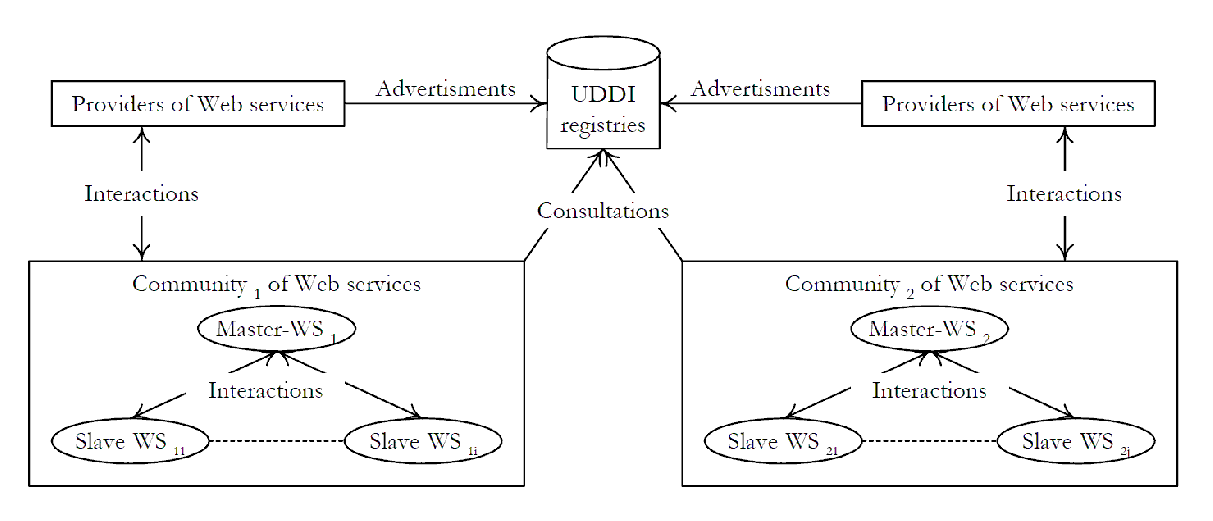
\includegraphics[width=16cm]{Figures/wsarch.eps}\label{wsarch}
            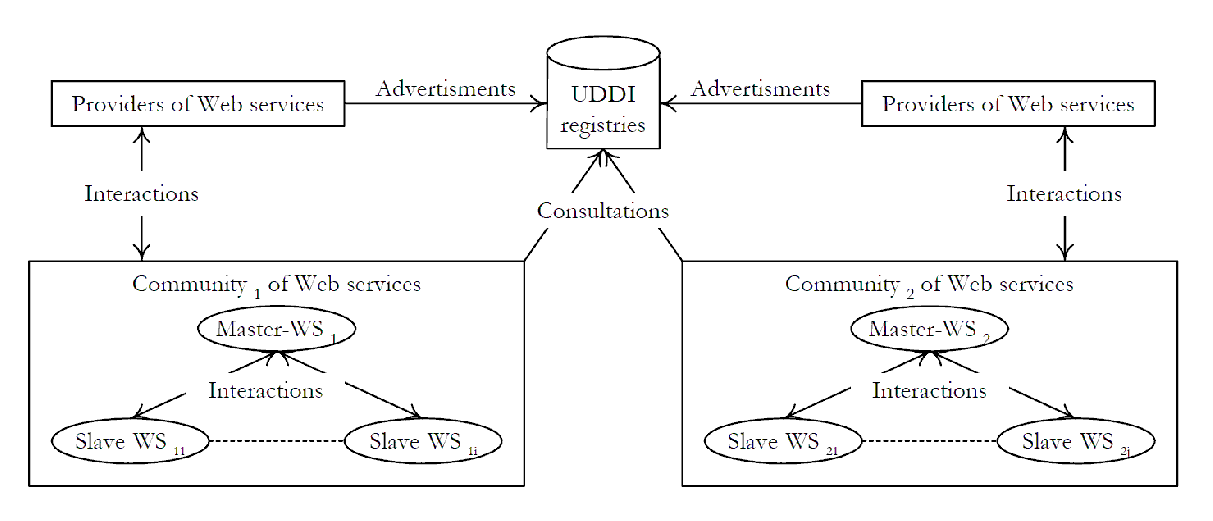
\includegraphics[width=16cm]{Figures/wsarch.eps}\label{wsarch}
            \caption{Communities of Web Services Architecture as Proposed in \cite{DBLP:journals/ijebr/MaamarSTBB09}}
            \end{center}
        \end{figure}

        Figure \ref{wsarch} depicts the basic architecture of communities of web services. The main components of the architecture are: 1) the providers of web services,
        2) UDDI registries and 3) communities of web services. Communities abstract the same model of defining, announcing and invoking of web services. They also adopt the same protocols that standard web services use with UDDI registries. UDDI is a platform-independent XML based registry list which facilitates worldwide web service discovery.

        The master web service is responsible with communication with web service providers and discovery registries. It it responsible for task distribution, web service selection,
        community management, maintaining a healthy set of web services satisfying end users requests with high QoS. In communities, the masters web services can be
        dedicated web services playing the master role during the entire time of being in the community. This master web service is independently developed and never
        participates in any composition. The master web services can also be chosen out of normal web services already inside the community \cite{DBLP:journals/ijebr/MaamarSTBB09}.


    \section{Cooperative Game Theory and Multi-agent Systems}\label{sec:CGTMS}


%        Cooperative game theory provides a set of mathematical and optimization tools for multi-agent environments. These tools have been utilized in communication networks and service oriented computing literature, where nodes as rational agents try to reason strategically and maximise their benefit.

        Cooperative game is a branch of game theory that studies
        strategies of self-interested entities or agents in a setting
        where those agents can increase their payoff by binding agreements
        and cooperating in groups. We let $N$ be a set of players. Any
        subset $S$ of $N$ can form a group called $coalition$. A
        \emph{coalitional game} is a pair $G = (N, v)$, where $v$ is called
        a \emph{characteristic function} $v: 2^N \to \mathbb{R}$, mapping the set of players of the
        coalition to a real number $v(S)$, the worth of $S$. This number
        usually represents the output or payoff or again the performance
        of these players working together as coalition.  If a coalition
        $S$ is formed, then it can divide its worth, $v(S)$ in any
        possible way among its members. The payoff vector $x \in
        \mathbb{R}^S$ is the amount of payoff being distributed among the
        members of the coalition $S$. The payoff vector satisfies two
        conditions:

        \begin{itemize}
            \item $x_i \geq 0$ for all $i \in N$, and
            \item $\sum_{i \in S} x_i \leq v(S)$
        \end{itemize}

        The second criteria is called the \emph{feasibility} condition,
        according to which, the payoff for each agent cannot be more than
        the coalition total gain. A payoff vector is also \emph{efficient}
        if the payoff obtained by a coalition is distributed amongst the
        coalition members: $\sum_{i \in S} x_i = v(S)$. This definition of
        the characteristic function works in \emph{transferable utility}
        (TU) settings, where utility (i.e., payoff) is transferable from
        one player to another, or in other words, players have common
        currency and a unit of income that is worth the same for all players
        \cite{myerson1991game}.

        When dealing with cooperative games, two issues need to be
        addressed:\\ 1. Which coalitions among all possible coalitions to form? \\
        2. How to reward each member when a task is completed?\\
        %
        The following sections help address these two issues.

        \subsection{Cooperative Game Concepts}


            {\bf Definition 1 (Shapley value)} Given a cooperative game $(N,
            v)$, the \emph{Shapley value} of player $i$ is given
            by\cite{shapley_value}:
            \begin{equation}\label{eq:shapley}
            \phi_i(N,v) = \sum_{S \subseteq N \backslash \left\{i\right\} }
            \frac{|S|! (|N|-|S|-1)!}{|N|!} (v(S \cup \left\{i\right\}) - v(S))
            \end{equation}

            \emph{Shapley value} is a unique and fair solution concept for
            payoff distribution among the members of the coalition. It
            basically rewards members with the amount of marginal contribution
            they have to the coalition.

            %\subsubsection{Core}

            {\bf Definition 2 (Core)} A payoff vector $x$ is in the $core$ of
            a coalitional game $(N, v)$ if and only if:
            \begin{equation}\label{eq:core}
            \forall S \subseteq N, \sum_{x_i \in S} x_i \geq v(S)
            \end{equation}

            The core is basically a set of payoff vectors where no subset of
            players $S^\prime$ could gain more than their current payoff by
            deviating and making their own coalition $\sum_{i \in S^\prime}
            x_i \geq v(S^\prime)$. The sum of payoffs of the players in any
            sub-coalition $S$ is at least as large as the amount that these
            players could earn by forming a coalition by their own. In a
            sense, it is analogue to Nash equilibrium, except that core is
            about deviations from groups of entities. The core is the
            strongest and most popular solution concept in cooperative game
            theory. However, its computation is a combinatorial problem and
            becomes intractable as the number of players increases. The core
            of some real-world problem games may be empty, which means having
            the characteristic function of the game $(N,v)$, there might be no
            possible distribution of payoff assuring stability of subgroups.

            {\bf Definition 3 (Convex cooperative games)} A game $(N,v)$ with
            characteristic function $v(S)$ is convex if:
            \begin{equation}\label{eq:convex}
            v(S) + v(T) \leq v(S \cup T) + v (S \cap T), \forall S,T \subseteq
            N.
            \end{equation}

            According to a classic result by Shapley \cite{S1971cores}, convex
            games always have a non-empty core. We will use a variation of
            convexity condition in our algorithm to check whether our
            coalitions are stable.

            \subsubsection*{$\epsilon$-core}\label{s:epsilon}
            %\emph{$\epsilon$-Core:}
            %\\
            When the \emph{core} set of a game is empty, it means no coalition
            of players can gain anything by deviating. An outcome would be
            unstable if a coalition can benefit even by a small amount from
            deviating, which is a strong requirement. In fact, in some
            situations, deviations can be costly, or players may have loyalty
            to their coalitions, or even it can be computationally intractable
            to find those small benefits. It would only make sense for a
            coalition to deviate if the gain from a deviation exceeds the cost
            of performing the deviation. \emph{$\epsilon$-core} relaxes the
            notion of the core, and only requires that no coalition would
            benefit significantly, or within a constant amount($\epsilon$) by
            deviating (see Equation \ref{eq:core}).

            \begin{equation}\label{eq:core2}
            \forall S \subseteq N, \sum_{x_i \in S} x_i \geq v(S) - \epsilon
            \end{equation}

            \subsubsection*{Coalition Structure Formation}\label{sec:coalition}

            Coalition structure formation is the problem of finding the best
            partition of web services into teams. In these settings, the
            performance of an individual service is less important than the
            \emph{social welfare} of the whole system, which is the sum of the
            values of all teams. Having the game $(N,v)$, a coalition
            structure $(CS)$ is \emph{socially optimal} if $CS$ belongs to set
            $\operatorname*{arg\,max}_{CS} v(CS)$ where $v(CS)$ is the sum of
            the values of all coalitions inside $CS$. $v(CS) = \sum_{C \in
            CS}v(C)$.
            %The outcome of a characteristic function game in coalition structure settings, consists of two parts; first a disjoint partition of players (agents) into coalitions, called a \emph{coalition structure} (CS) and second a \emph{payoff vector} as mentioned in cooperative game solution concepts, which distributes the value of each coalition among its members.


        \subsection{Cooperative Game Examples}\label{sec:CWSDefinition}

        \emph {THIS EXAMPLE IT NOT COMPLETE YET}

        An example which has closely resembles our community service model is the \emph{Single landowner and landless workers} example.
        This example was introduced in \cite{GVK369342747} and represents the \emph{landowner} entity which is providing jobs and \emph{landless workers} who cannot do anything by themselves and need to work with a landowner to gain revenue (payoff).

        In this game, land is owned by a single person, the \emph{landowner}. We refer to the other people as \emph{workers}. In this case we have a game there the set of players are the landowner and the $m$ workers, possible actions for coalitions with only workers would be distributing the zero output for all where no member receives any output. The set of actions of a coalition $S$ consisting of the landowner and $k$ workers would be the set of all $S$-allocations of the output $f(k+1)$ among the members of $S$. The preference of each player would be the amount of out she obtains.

        In this game the action $a_{N}$ of the grand coalition in which the landowner obtains all the output $f$(n)
        is in the core: all coalitions that can produce any output include the landowner, and none of these
        coalitions has any actions that makes her better off than she is in $a_{N}$.

        For any value of n The core contains actions in which the workers receive some output.
        The workers need the landowner to produce any output, but the landowner
        also needs the workers to produce more than $f$(1), so stable actions of the grand coalition exist in which the
        workers receive some output. Take the landowner to be player 1, and consider the action $a_{N}$ of the grand
        coalition in which each player $i$ obtains the output $x_{i}$, where $x_{1}+...+x_{n}=f(n)$. Under what conditions
        on  $(x_{1},..,x_{n})$ is $a_{N}$ in the core? Because of my assumption about the shape of the function $f$, the
        coalitions most capable of profitably deviating from $a_{N}$ consist of the landowner and every worker but one.
         Such a coalition can, by itself, produce $f(n-1)$, and it may distribute this output in any way among its members.
         Thus for a deviation by such a coalition not to be profitable, the sum of $x_{i}$ and any collection of $(n-2)$ other
          $x'_{i}$s must be at least $f(n-1)$. That is, $(x_{1}+...+x_{n})-x_{i}\geq f(n-1)$ for every $j=2,..,n$. Because
          $x_{1}+...+x_{n}=f(n)$, we conclude that $x_{i}\leq f(n)-f(n-1)$ for every player $j$ with $J\geq 2$ (i.e. every worker).
          That is, if $a_{N}$ is in the core then $0\leq x_{j}\leq f(n)-f(n-1)$ for every player $J\geq 2$. In fact, every such action
          is in the core, as you are asked to verify in the following exercise.

%          Core of landowner-worker game: Check that no coalition can improve upon any action of the grand
%          coalition in which the output received by every worker is nonnegative and at most $f(n)-f(n-1)$. (Use the fact that
%          the form of $f$ implies that $f(n)-f(k)\geq (n-k)(f(n)-f(n-1))$ for every $k\leq n$.)

%          We conclude that the core of the game is the set of all actions of the grand coalition in which the output $x_{i}$
%          obtained by each worker $i$ satisfies $0\leq x-{1}\leq f(n)-f(n-1)$ and the output obtained by the landowner is the
%          difference between $f(n)$ and the sum of the worker's shares. In economics jargon, $f(n)-f(n-1)$ is a worker's
%          ``marginal product". Thus in any action in the core, each worker obtains at most her marginal product.

%          The worker's shares of output are driven down to at most $f(n)-f(n-1)$ by competition between coalitions consisting
%          of the landowner and workers, in cahoots with the landowner, can deviate and increase their share of output. That is,
%          each worker's share of output is limited by her comrade's attempts to obtain more output.

%          The fact that each worker's share of output is held down by interworker competition suggests that the workers might
%          be better off if they were to agree not to join deviating coalitions \emph{except as a group}. You are  asked to check
%          this idea in the following exercise.

        %\subsection{Cooperative Games in Service Oriented Computing}\label{sec:CWSArchitecture}

        \subsection{Representation and Complexity issues}\label{sec:CWSArchitecture}

        Shapely value is the unique "fair" way to distribute the total surplus generated by the coalition, among all the players.
        The nature of the Shapley value is combinatorial, as all possible orderings to form a
        coalition needs to be considered. This computational complexity can sometimes be
        an advantage as agents cannot benefit from manipulation. For example, it is NP-complete
        to determine whether for a bunch of agents to collude and make their own coalition and guarantee
        an increase in payoff of all participants\cite{conf/aaai/YokooCSOI05}.
        There are some representations that allow to compute the Shapley value efficiently by reducing the input size of the problem.
        One example is \emph{Induced subgraph games}
        which was introduced by Deng and Papadimitriou \cite{Deng94}. In this representation, players are represented by graph nodes, and
        their valuation function should be sum of weights all edges between the node and all its neighbors. It is a succinct representation, using
        an adjacency matrix, which need only $O(n^2)$ space to store all the input, which is a big reduction from $O(2^n)$.
        if weights of all the edges in graph are all positive, the Shapley value can be computed in $O(n^2)$ time.
        However, this representation is not complete, some games cannot be represented by a induced subgraph game\cite{conf/aaai/YokooCSOI05}.

        Ketchpel introduces the Bilateral Shapley Value (BSV)\cite{conf/aaai/Ketchpel94a} for coalition games with general valaution functions.
        It reduces the combinatorial complexity of the computation of the Shapley value, breaking the community to multiple disjoint set.
        With backtracking and dynamic programming like methods, they merge and store the marginal contribution of disjoint coalitions,
        reducing the overall complexity of the algorithm. However, the solution is still NP-Complete and BSV time and space complexity grows exponentially.

        In order to make cooperative game concepts practical in real world application, we have proposed an approximation multi-layer
        algorithm useful for service orinted computing settings. Our excrements illustrate, these algorithms can provide
        applicable and near optimal solutions for real world applications.


    \section{Related Work}\label{sec:BRRelatedWork}

        One of the first contributions in which web service community was introduced was in \cite{Zeng:2003:QDW:775152.775211}. They defined web service community as collection of web services providing same functionality however with different quality metrics.

        Medjahed and Boubuettaya \cite{journals/dpd/MedjahedB05} have proposed a framework and a community builder mechanism which uses semantic analysis, providing an ontological organization of web services having same domain of interest. The community builder would suggest web services having similar operations with any community to join the community, or form their own communities in case the semantic analysis cannot find any community with close enough operations and service types.

        Most of the recent work on communities of services are either
        user-centric and focus on user satisfaction
        \cite{Chun02user-centricperformance} or system-centric and focus
        on the whole system throughput, performance and utilization. There
        are many contributions in distributed, grid, cluster and cloud
        services which are system-centric. However, in real world
        environments and applications, both users and service providers
        are self-interested agents, aiming to maximize their own profit.
        In those environments, both parties (users and services) will
        collaborate as long as they are getting more benefits and payoff.

        In this direction, recently \cite{DBLP:conf/IEEEscc/LimTMB12,
        DBLP:conf/IEEEscc/KhosravifarABT11, 10.1109/TSC.2012.12} proposed mechanisms to help
        users and services to maximize their gain. A two-player
        non-cooperative game between web services and community master was
        introduced in \cite{DBLP:conf/IEEEscc/KhosravifarABT11}. In this
        game-theoretic model, the strategies available to a web service
        when facing a new community are requesting to join the community,
        accepting the master's invitation to join the community, or
        refusing the invitation to join. The set of strategies for
        communities are inviting the web service or refusing the web
        service's join request. Based on their capacity, market share and
        reputation, the two players have different set of utilities over
        the strategy profiles of the game. The main limits of this game
        model are: 1) its consideration of only three quality parameters,
        while the other factors are simply ignored; and 2) the
        non-consideration of the web services already residing within the
        community. The game is only between the community master and the
        new web service, and the inputs from all the other members are
        simply ignored. The consideration of those inputs is a significant
        issue as existing web services can lose utility or payoff because
        of the new member, which can results in an unhealthy and unstable
        group. The problem comes from the fact that the existing members
        should collaborate with the new web services, so probably their
        performance as a group can suffer. Existing members may even
        deviate and try to join other communities if they are unsatisfied.
        Those considerations of forming stable and efficient coalitions
        are the main contributions of this research work.

        In \cite{DBLP:conf/IEEEscc/LimTMB12}, a 3-way satisfaction approach
        for selecting web services has been proposed. In this approach,
        the authors proposed a web service selection process that the
        community masters can use. The approach considers the efficiency
        of all the three involved parties, namely users, web services and
        communities. In this work, it is shown how the gains of these
        parties are coupled together using a linear optimization process.
        However, the optimization problem in this solution tends to
        optimize some parameters considering all web services regardless
        of their efficiency and contribution to the community's welfare.
        Moreover, there are no clear thresholds for accepting or rejecting
        new web services. The solution of the optimization problem could,
        for instance, suggest web services already residing within the
        community to increase or decrease their capacity to cover up the
        weakness of other parties in the system. However, a high
        performing web service could deviate anytime it finds itself
        unsatisfied within the community instead of adjusting its service
        parameters.

        In \cite{10.1109/TSC.2012.12}, a cooperative scheme among autonomous
        web services based on coalitional game theory has been introduced. They have proposed an algorithm to
        reach individually stable coalition partition for web services in order to
        maximize their efficiency. The communities choose new web services on the promise
        that it would benefit the community without decreasing any other web service's
        income. In their model, the worth of community is evaluated with high emphasis on
        availability metric and considering price and cost values only. The community structure is based on a coordination chain,
        where a web service is assigned as a \emph{primary} web service and the community task destribution
        method, will initially invoke the primary web service and only if the primary web service is unavailable
        will invoke the next backup web services as they are ordered in the coordination chain. However in cooperative models, it is preferred to
        have a real and active cooperative activity engaging all agents to perform the tasks more efficiently. Especially nowadays
        with recent advancement in cloud and hardware infrastructures availability is becoming less of an issue. So the backup web services
        in their model have a very low chance of getting jobs, especially the ones further in chain, which is huge waste of web services
        capabilities.


        % THIS IS REPEATED
        \emph {-- this is repeated --}
        In this research work, we use game theory to
        propose a cooperative game model for the aggregation of web
        services within communities. The solution concepts of our
        cooperative game seeks to find efficient ways of forming
        coalitions (teams) of web services so that they can maximize their
        gain and payoff, and distribute the gain in a fair way among all
        the web services. Achieving Fairness when the gain is distributed
        among the community members is the main factor to keep the
        coalition stable as no web service will expect to gain better by
        deviating for the community. In other words, the coalition is made
        efficient if all the members are satisfied. We first propose a
        representation function for communities of web services based on
        their QoS attributes. By using this function, we can evaluate the
        $worth$ of each community of web services. When facing new
        membership requests, a typical community master checks whether the
        new coalition having the old and new set of web services will keep
        the community stable or not. The community master will reject the
        membership requests if it finds out that the new coalition would
        be unstable, preventing $any$ subset of web services from gaining
        significantly more by deviating from the community and joining
        other communities or forming new ones. The computation of
        solutions for cooperative game theory problems is combinatorial in
        nature and proven to be NP-complete \cite{Algorithmic}, making
        this computation impractical in real world applications. However,
        using the concepts of coalition stability, we propose
        approximation algorithms running in polynomial time providing web
        services and community masters with applicable and near-optimal
        decision making mechanisms.




%*******************************End Background **********************************

\setcounter{chapter}{2}

\chapter{Coalition Formation for Autonomous Web Services}\label{sec:coalitionformationws}

In this chapter, we present our coalition model of agent-based web
services within communities\cite{SCC2013efficient}. We start by describing the general
architecture and considered parameters for web services.
Thereafter, problem modeling and formulation will be introduced in
terms of task distribution and community revenue. Web service
cooperative games in different settings will follow along with
some simulation results.

\section{Preliminaries}\label{s:preliminaries}

Our system consists of three main types of entities working
together: \emph{1) Web services} are rational entities that aim to maximize
their utilities by providing high quality services to end users.
They aim to maximize their individual income by receiving enough
requests from end users. In order to increase their revenue, web
services seek for more tasks if they have the capacity and
throughput to do so. Web services can join communities to have
better efficiency by collaborating with others, to have access to
higher market share, and to have opportunity of receiving a bigger
task pool from end users. Throughout this proposal, in our
equations, we refer to web services as $ws$ and to the set of web
services hosted by a given community as $C$. 
%To simplify the
%notation, sometimes we simply write $ws$ instead of $ws \in C$ to
%go through the elements $ws$ of the set $C$.
\emph{2) Master Web Services} or the community coordinators, are representatives of the
communities of web services and responsible for their management.
Communities receive requests from users and aim to host a healthy
set of web services to perform the required tasks. They seek to
maximize user satisfaction by having tasks accomplished according
to the desired QoS. 
%In fact, higher user satisfaction will bring
%more user requests and increase the market share and revenue of
%the community. 
\emph{3) Users} generate requests and try to find the best
available services. User satisfaction is abstracted as function of
quantity and quality of tasks accomplished by a given service.
Higher user satisfaction leads to higher trust of the community by users hence directing more requests towards that service provider.

Web services come with different quality of service parameters.
These parameters include availability, reliability, successability, throughput, latency, capacity, cost, regulatory and security\cite{DBLP:conf/smc/Al-MasriM09a}.
We adopted a real world dataset \cite{DBLP:conf/smc/Al-MasriM09a}
which has aggregated and normalized each of these parameters to a
real value between 0 and 1. Since requests are not shared among
web services and are distributed among all of them inside a
community, each one of them comes with a given QoS denoted by
$(QoS_{ws})$. We assume that $(QoS_{ws})$ is obtained by a certain linear weight function of the parameters. We use this quality output later in evaluating the
community \emph{worth} or \emph{payoff} function.

Figure 3 represents our revised architecture of web service
communities where tasks are to be distributed among the members
that are interested in forming stable coalitions. As discussed in
Chapter 2, communities are essentially virtual platforms
aggregating web services having similar and complementary
functionalities and communicate with other entities such as UDDI
registries and users using particular protocols. Web services join
communities to increase their utility by having larger market
share and task pool. 
%Community coordinators or master web services
%are responsible for community development, managing membership
%requests from web services and distributing user tasks among the
%community members. Community coordinators try to attract quality
%web services and keep the community as stable and productive as
%possible to gain better reputation and user satisfaction, which
%results in having higher revenue.

\begin{figure*}[!t]
\centerline{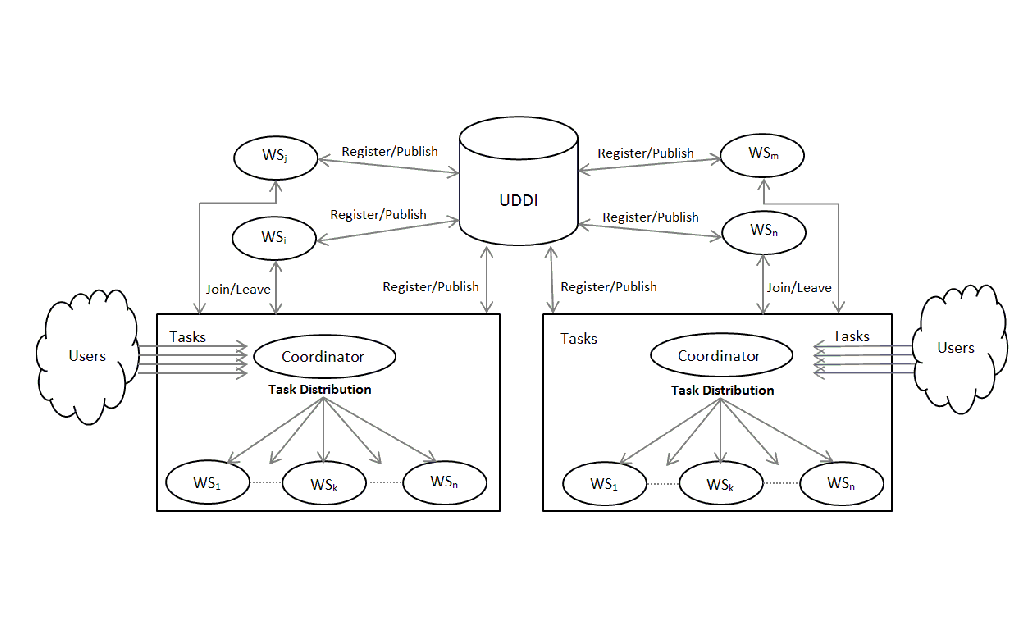
\includegraphics[width=15cm]{community.eps}}
\caption{Architecture of Web Service communities}
\label{fig_community}
\end{figure*}


\section{Problem Formulation and Modeling}\label{s:model}

In this section, we present  web services and community coordinator's interactions, the task distribution process and revenue models in web service communities.

\subsection{Task Distribution}

As mentioned in Section \ref{s:preliminaries}, communities
are robust service providers with well established market share
and reputation. By maintaining their reputation and performance,
they attract  end users which choose them as service providers to
perform their tasks. The community master is characterized by a
request rate $(R_C)$ from users. Each web service comes with a
given QoS ($QoS_{ws}$) from which the throughput $Th_{ws}$ is
excluded. Throughput is the average rate of tasks a web service
can perform per time unit. Its exclusion from $QoS_{ws}$ allows us
to build our analysis on the particular value of $Th_{ws}$. Thus,
web services perform tasks with an average output quality of
$QoS_{ws}$ and a throughput rate of $Th_{ws}$.

The community master uses a slightly modified \emph{weighted fair queuing} method to distribute tasks among its members. The goal is to allocate incoming tasks to web services with a rate matching the throughput value of $Th_{ws}$. In \emph{weighted fair queuing} method \emph{all} the input flow is multiplexed along different paths, however in our case if the input rate $(R_C)$ of the community is more than the summation of throughput values of the web services in the community, some of the input tasks will be queued and served with delay. Thus, the amount of tasks performed by community is $\sum_{ws \in C}{(Th_{ws})}$ when $\sum_{ws}{Th_{ws}} \leq R_{C}$. However, when the input rate $(R_C)$ of the community is less than the summation of throughput values of the web services in the community,
%the community has more web services having more total throughput value than community's request rate
$(R_C)$ the \emph{weighted fair queuing} algorithm assigns a weighted task rate of $R_C \times \frac{Th_{ws}}{\sum_{ws}{Th_{ws}}}$ for each web service ($ws$) and the total rate of tasks being performed is $R_C$, the community's receiving request rate.

While distributing tasks, the community master can verify the performance, throughput and quality of service of   tasks being performed by web services. It can recognize if web services are capable of doing the amount of tasks they advertised. If for any reason there is a decline in quality metrics or throughput, the  community master will announce the new parameters and community masters and members can consider those values as benchmark for future performance calculations but also to penalize them.
In this way, players have incentive to reveal their real capabilities to profit best from the community and to avoid being penalized. In addition, the system should be dynamic enough to detect and react to web services quality metrics variation as over time web service metrics may  degrade or improve, a change that the community should adjust to.
% Therefore its easy for the system to encourage players to be in some sense incentive compatible in the way that they would profit best by truthfully revealing their capabilities. Also it is important to be dynamic enough to consider web services which may have their quality metrics degraded or even improved over time for any reason and be able to adjust the community with new parameters.

\subsection{Community Revenue}

The communities and web services earn revenue by performing tasks.
The total gain is function of quality ($QoS_{ws}$) and throughput
($Th_{ws}$) of tasks being performed. We have adopted a linear equal weight average over
the QoS parameters excluding the
$Throughput$ and $Cost$ parameters. A community has the option to
weigh specific QoS parameters depending on the expectations of
their clients.

The maximum potential output of a community $(PO(C))$  is an aggregation of number of tasks, times their quality, for each web service member of the community:

\begin{equation}
PO(C) = \sum_{ws \in C}{(T_{ws} \times QoS_{ws})}
\end{equation}

If the summation of throughput values ($Th_{ws}$) of community members exceeds the input task rate of the community ($R_C$) the community cannot perform at its maximum potential. It denotes the case when the community has more web services than it needs to perform the input task load. The actual output has to be normalized to the amount of tasks being performed.

\begin{equation}\label{out_c}
Out(C) = \left\{
  \begin{array}{l l}
    PO(C) & \quad \text{if $\sum_{ws}{Th_{ws}} \leq R_{C}$}\\
    PO(C) \times \frac{R_{C}}{\sum_{ws}{Th_{ws}}} & \quad \text{if $\sum_{ws}{Th_{ws}} > R_{C}$}
  \end{array} \right.
\end{equation}

The revenue function of the web service community is a linear function of $Out(C)$ with a positive constant multiplier.


 \section{Web Service Cooperative Games}\label{s:game_solution}

In this section, we present different web service community models
and focus on the problem of how both web services and community
masters as rational entities would adopt strategies to maximize
their payoff.

\subsection {Web Services and One Community}

In this scenario, we assume the existence of a typical community
managed by its master, and web services need to join it to be able
to get requests from the master. The community master is
characterized by a requests rate $(R_{C})$ from users. Each web
service comes with a given QoS ($QoS_{ws}$). The worth of a community
$v(C)$ is set to Out(C) based on equation \ref{out_c}.

As mentioned in previous section, the worth and output of a
community  is a function of the
throughput and provided QoS of its web service members. If the throughput rate is more than
the master's input request rate, it means the web services inside
the community are capable of serving more requests than the
demand. Considering this factor, the valuation function is
designed to balance the output performance so that it matches the
exact throughput rate and QoS the web service can provide within
the particular community.
%** In the case where the limited tasks are distributed among web services uniformly, the value of coalition would be the proportion of the average QoS times their throughput to rate of available requests. **

In this first scenario, we only consider one grand coalition and
analyze the system from the point of view of one single master web
service and a collection of web services. The master web service
decides which members can join
%or should leave%
the community and distributes the requests and income among its
community members.

%\begin{figure}[!t]
%\centering
%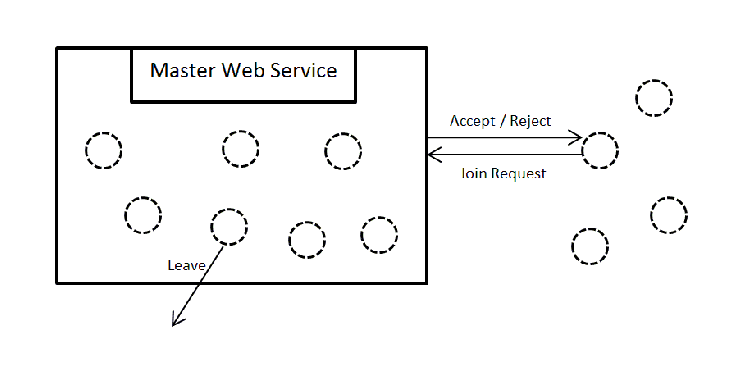
\includegraphics[width=3in]{Figures/s1.eps}`
%\caption{Web Services and A Grand Community}
%\label{fig_sim1}
%\end{figure}

The membership decision is made based on throughput and \emph{QoS}
of the considered web service. The goal is to have quality web
services in the community so it stays stable and no other web
services would have incentives to deviate and leave the coalition
$C$. Therefore, a basic method would be to check the core of the
coalition $C$ considering all the current community members (all
web services already residing within the community) and the new
web service. This algorithm uses the \emph{Shapley value}
distribution method as described in Equation \ref{eq:shapley} to
distribute the gain of $v(C)$ among all the members and then
checks if the \emph{Shapley value} payoff vector for this
community having the characteristic function $v(C)$ is in the
\emph{core}. In the \emph{Shapley value} payoff vector, the payoff
for each web service $ws_i$ is calculated based on its marginal
contribution $v(C \cup {i}) - v(C)$ over all the possible
different permutations in which the coalition can be formed, which
makes the payoff distribution fair. Because of going through all
the possible permutations of subsets of $N$, the nature of the
\emph{Shapley value} is combinatorial, which makes it impractical
to use as the size of our coalitions grows. However, it is proven
that in convex games, the \emph{Shapley value} lies in the core
\cite{DBLP:conf/ijcai/GrecoMPS11, myerson1991game}. Thus, if the
\emph{Core} is non-empty, the payoff vector is a member of the
\emph{Core}. The following proposition is important to make our
algorithm tractable.


\subsection {Web Services and Many Communities}

In this scenario, we consider multiple communities managed by
multiple master web services, each of which is providing
independent request pools. Identical
to the first scenario, master web services form coalitions with
web services. We use coalition structure formation methods to
partition web services into non-empty disjoint coalition
structures. As mentioned in Section \ref{sec:coalition}, the used
algorithms in \cite{Sandholm:1999:CSG:317145.317152,DBLP:conf/ijcai/GrecoMPS11,DBLP:conf/ijcai/RahwanMJ11} try to
solve key fundamental problems of what coalitions to form, and how
to divide the payoffs among the collaborators.

%\begin{figure}[!t]
%\centering
%\includegraphics[width=3in]{Figures/s2.eps}
%\caption{Web Services and Many Communities}
%\label{fig_sim2}
%\end{figure}

In coalition-formation games, formation of the coalitions is the
most important aspect. The solutions focus on maximizing the
social welfare. For any coalition structure $\pi$, let
$v_{cs}(\pi)$ denote the total worth $\sum_{C \in \pi}{v(C)}$,
which represents the \emph{social welfare}. The solution concepts
in this area deal with finding the maximum value for the social
welfare over all the possible coalition structures $\pi$. There
are $centralized$ algorithms for this end, but these approaches
are generally NP-complete. The reason is that the number of all
possible partitions of the set $N$ grows exponentially with the
number of players in $N$, and the centralized algorithms need to
iterate through all these partitions.
%These algorithms \cite{DBLP:conf/ijcai/GrecoMPS11, DBLP:conf/ijcai/RahwanMJ11, RePEc:wpa:wuwpga:0110001} are centralized algorithms, where all the complexity. However these algorithms are more intractable than Core stable solutions and practical with some constraints in practice\cite{RePEc:wpa:wuwpga:0110001}.
In our model, we propose using a distributed algorithm where each
community master and web service can be a decision maker and
decide for its own good. The aim is to find less complex and
distributed algorithms for forming web services coalitions
\cite{DBLP:journals/igtr/AptW09,Dieckmann02dynamiccoalition,ray2007game}.
The distributed merge-and-split algorithm in
\cite{DBLP:journals/igtr/AptW09} suits our application very well.
It keeps splitting and merging coalitions to partitions which are
preferred by all the players inside those coalitions.


\section{Taxation, Subsiding and Community Stability}\label{s:tax}

We discussed $core$ as one of the prominent solution concepts in
cooperative games. Working together, completing tasks and
generating revenue, agents need to distribute the gain in a way no
agents would gain more by forming their own group. However, in
most cases, the core of a game is empty, so we introduced the
\emph{$\epsilon$-core} concept, where agents would only earn a
minimal amount of $\epsilon$ by deviating from the coalition.
Stability is an attractive property for communities. In addition,
communities would benefit by having slightly more web services
than the exact number of web services needed to satisfy the task
rate cap. This is because there is always a possibility that the
web services may leave the community or they may under perform and
degrade the quality values they were initially performing with.

The solution we propose for communities to ensure stability is
applying a tax $\epsilon$, which is an amount of cost for those
web services that decide to change communities (let us say from
$C$ to $C'$), which would make deviation a costly act. However,
this would require all the community coordinators to agree on a
same amount of taxation, being governed by some external entities;
otherwise, web services would join communities charging the lowest
amount of tax. Before deciding to change the community, each web
service $i$ has to be sure that the gain $g_i(C \rightarrow C')$
calculated in Equation \ref{eq:gainsh} based on the Shapley values
of $i$ in the previous and new communities and the tax $\epsilon$
is positive, which means, what the web service would gain in $C'$
is greater than what it gains in $C$ and the tax it would pay if
moving all together:


\begin{equation}\label{eq:gainsh}
g_i(C \rightarrow C') = \phi_i(C',v) - \phi_i(C,v) - \epsilon
\end{equation}


Another viable solution we introduce to our scenario is to
stabilize the game using external subsidies. The reason a game is
not stable is that the community is not making enough revenue to
allocate enough gain to the players. A community coordinator can
subside its community with a constant coefficient value of
$\lambda$.
%
%Rewarding a community with high number of quality participants
%with $\lambda v(C)$, where $\lambda \leq 1$.
%
Obviously, with a big value for $\lambda$, it is always possible
to stabilize the community. However, this can be a costly act for
the community coordinators, so they are interested in the minimum
subside value of $\lambda$ making the community stable. This can
be achieved by solving the following linear program:
%
  \begin{alignat*}{3}
    \min~   & \lambda  \\
    \text{s.t. } & \lambda v(C) > v(C') & ~& \text{ for all } C' \subset C
  \end{alignat*}


%When a new web service $i$, wants to join the community, the
%valuation function of the community members and the new web
%service is subsided by the community coordinator in order to
%incentivize formation of this community and is set to:
%\begin{equation}\label{eq:taxv}
%v'(C \cup \{i\}) = \lambda \times v(C \cup \{i\})
%\end{equation}
%In equation \ref{eq:taxv} the value of $v'$ is
%replaced with the valuation function for the new forming coalition
%$C \cup \{i\}$.
Subsiding or taxing in order to reduce the
bargaining power of sub coalitions are called $taxation$
\cite{eps346856} methods. We evaluate the effectiveness of these
two methods experimentally through extensive implementations in
the next section.



%Thus, another way to garantee \emph{$\epsilon$-core} stability can be achieved by some surplus payments from community coordinators. These concepts of applying cost in coallition values in order to reduce their bargaining power are called $taxtation$ methods\cite{eps346856}.

%The \emph{$\epsilon$-core} concept, in its definition, considers the willing to join or deviate from agent's point of view. It claims agents for any reason will be not willing to deviate to gain less than $\epsilon$ amount of profit. Communities can agree on However, in our case, the community master is willing to keep web services in communities too. There are several reasons for this, one reason is there is always possibility that agents may leave the community or they may under perform from the quality values they were initially performing with. To this end, our communities will reward and valuate web services in the community

\section{Competitive behaviour of services within communities}\label{s:coop}

In previous sections, our focus was on community formation and we emphasised on cooperative behaviour of the web services as agents. Within communities, those services, selfish and utility maximizers by nature, can follow two different strategies, namely cooperation and competition in order to increase their payoffs when they provide services to consumers \cite{VuFind-10008938119}. In typical business settings, services are used to compete within communities as they provide the same functionalities and the number of users requests is finite. However, the same reason of providing similar functionalities can lead services to cooperate because they can replace each other in case of failure or unavailability, and services can do better in a coalition structure. Analyzing services competition and cooperation strategies within communities is still an open problem that motivates the research described in this section. we propose a mechanism within which service agents
in the community could choose either to compete for an announced task\footnote{Requests and tasks are used in this paper interchangeably.}, or to cooperate with other competing services in the same community to accomplish some subtasks of the announced task. We equip intelligent web services to follow a reasoning technique to choose best interactive strategy (Coopetitive attitude, which is categorized to compete and cooperate). In the proposed system, We explore details behind the strategic decision making procedures and enable service agents to apply different techniques to constrain high efficiency and obtain the maximum utility. We investigate services' expected payoffs and the involved probabilities that are used to choose over the two interacting strategies.









\subsection{The Proposed Framework}\label{The Proposed Framework}
In this section, we first present the architecture of the proposed
model. We explore the characteristics of intelligent service
agents and their network. We link this architecture to the
implemented system where we investigate the services' coopetitive
attitudes. We compute the involved system parameters and explain
the services' interactive strategy profiles by highlighting their
coopetitive choices.

\begin{figure}[h]
\centering
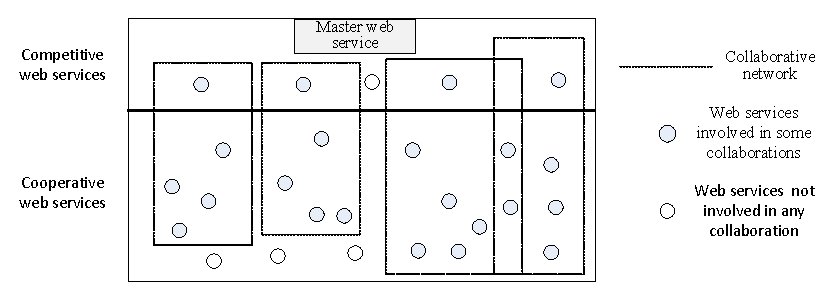
\includegraphics[scale=1]{architecture++.eps}
\caption{Services are partitioned into competitive and cooperative
sets. Competitive services may get tasks directly from the master
agent and they can share it with other cooperative services in
their collaborative networks within the same community.}
\label{architectureFigure}
\end{figure}

\subsubsection{The Architecture}

Figure \ref{architectureFigure} illustrates the architecture of a
typical community aggregating a number of services with different
interactive strategies. Some of them compete for the task where
they directly deal with the master. Some others cooperate in the
associated task where they only deal with the competed service as
the task leader and do not directly interact with the master (the
master deals only with the service that has bid for the task,
which is responsible of choosing its collaborative network). In
both sets, some service agents are for certain moments out of any
collaboration network. Upon allocation of
the task, the service is responsible for offering the required QoS
that is stated in the task being generated by a consumer.
Afterwards,  the master rewards or penalizes the competing
service by upgrading or degrading its reputation according to the
offered QoS compared with the required one. This comparison
influences the sorting mechanism used by the master to allocate
the tasks in further task allocation rounds.


%ok til here


\subsubsection{System Parameters}
In this section, we demonstrate the involved parameters and their
corresponding formulations and explanations.

\textbf{Task QoS} ($T_{QoS}^r$) is the required QoS metric for a
specific task $r$. Users define tasks with specific QoS
requirements such as response time, availability, and
successability (or accuracy). We aggregate and
normalize these metrics to a value between $0$
and $1$. %Throughout this paper, we refer to this value as
%$T_{QoS}$.

\textbf{Service QoS} ($QoS_w^r$) is the QoS provided by the
service $w$ after performing the task $r$. Again, the metrics that
contribute in computing this QoS are aggregated and normalized to
a value between $0$ and $1$. The offered quality might or might
not meet the required task quality $T_{QoS}^r$. In the latter
case, the service user would be disappointed and a negative
satisfaction feedback is expected. In our proposed system, both
cases are considered when calculating the services' reputation.

%\textbf{NTD} is the number of tasks completed by a web service.

\textbf{Budget} ($B_w^t$) is the amount of money the service agent
$w$ has in its disposal during the window time $t$ (i.e.,
$[0,t]$), which helps pay for the community membership fees
($\epsilon$) and is one of the parameters that the service agent
considers when deciding about getting involved in a competition or
not.

\textbf{Reputation} ($Rep_w^t$) is a significant factor in any
online community \cite{Fouss:2010:PRM:1751668.1751727}. Without a reputation enabling
mechanism, users cannot differentiate among services, specially
the ones which offer the same type of service. Reputation
mechanisms usually aggregate users' experiences and in our case it
strongly depends on QoS that each service provides. Users define
tasks, each one with specific quality $T_{QoS}^r$, so that after
performing a certain number of tasks, each one with $QoS_w^r$,
during a window time $t$, the reputation of $w$ gets evaluated by
the master agent. $Rep_{w}^{t}$ refers to the reputation of $w$
during that window time $t$.

In Equation \ref{repr}, we compute the reward that the master
computes considering the task $r$'s QoS $T_{QoS}^r$ compared with
the service offered quality $QoS_w^r$. In case the offered quality
meets user expectations, the reward value would be positive. In
this system, we consider a small value as default rewards $\eta$
which the master considers together with the proportional level of
satisfaction as a weighted value (by $\upsilon$). In this case,
the higher the offered quality, the more weighted reward. In case
the offered quality did not meet the user expectations, the reward
would be negative. A default penalty value $\rho$ (where
$\rho>\eta$) together with the weighted proportional difference
are therefore considered. The idea is to harshly penalize the
services rather than rewarding them. To this end, rational service
agents should carefully analyze their capabilities once the
available tasks are announced. Equation \ref{reward} computes the
obtained reward by $w$ during the window time $t$ considering the
set $task_w^t$ of tasks performed by $w$ during the window time
$t$. In our proposal, service agents have the goal of increasing
their budget, which is directly related to their reputation. Thus,
they have to decide strategically how to maximize this value.

\begin{equation} \label{repr}
reward_w^r = \begin{cases}
\eta + \upsilon \frac{QoS_w^r}{T_{QoS}^r+QoS_w^r}   & \text{if $T_{QoS}^r\leq QoS_w^r$;}\\
-(\rho +  \upsilon \frac{T_{QoS}^r}{T_{QoS}^r+QoS_w^r} ) & \text{otherwise.}\\
\end{cases}
\end{equation}


\begin{equation} \label{reward}
reward_w^t =
\begin{cases}
\frac{\sum_{r \in
task_w^t}reward_w^r}{|task_w^t|}& \text{if $task_w^t \neq \emptyset$;}\\
0 & \text{otherwise.}\\
\end{cases}
\end{equation}

The assigned reputation value is updated by the computed reward
value. The computed reputation of services is bounded by the
minimum and maximum reputation values $0$ and $1$. % to constrain
%the balance the cooperative community of web services. The updated
%Let $\Gamma = Rep_{w}^{t} + reward_w^t$.
%The updated reputation
%value is then computed as follows:
%
%\begin{equation}\label{repz}
%%Rep_{w}^{t+1} = Rep_{w}^{t} + reward
%%\end{equation}
%%\begin{equation*}
%Rep_{w}^{t+1} = \begin{cases}
%
%\Gamma & \text{if $ 0 \leq \Gamma \leq 1$;}\\
%0  & \text{if $\Gamma < 0$;}\\
%1 & \text{if $\Gamma > 1$.}\\
%\end{cases}
%\end{equation}
%
%For new services with no previous reputation value, we use the
%bootstrapping trust technique proposed in \cite{conf/icwe/YahyaouiZ11}. This
%technique consists in giving the new services a chance and observe
%their behaviors for a period of testing time. The observation
%sequence is modeled as a hidden Markov model that is used to
%detect the behavior of the service by comparing the observation
%behavior against pre-defined trust patterns. Based on the matching
%result, an initial value is assigned to the service. Using this
%initial reputation value, services quickly converge to their
%actual and stable values using the update function.

%\begin{proposition}\label{Complexity-Rep}
%$Rep_{w}^{t}$ can be computed in time $O(|t|)$, i.e., in time
%linear in the size of the window $t$.
%\end{proposition}

%\begin{proof}\footnote{In this paper, we
%assume that the common arithmetic and elementary functions, such
%as multiplication, division and trigonometric functions can be
%computed in time $O(1)$ as they operate on inputs of fixed sizes.}
%The function $Rep_{w}^{t}$ is recursive on $t$, but the algorithm
%works by storing the last calculated reputation value in a
%variable, so it will not be recalculated again at each iteration.
%However, the calculation of $reward_w^t$ is needed. Since the
%function $reward_w^t$ can be computed in time linear in the number
%of tasks (see Equations \ref{repr} and \ref{reward}), which in
%turn is linear in the size of the window time, the result follows.
%$\Box$
%\end{proof}

\textbf{Growth Factor} ($G_w^t$) is a parameter which declares
services' performance based on their recent strategies and
activities. Growth factor is relative to services' reputation
$Rep_w^t$, QoS during the window time $t$ $QoS_w^t$, and budget
$B_w^t$. This factor is the main variable a typical service uses
to decide about which strategy to adopt. We use Equation \ref{eq:growthfactor} to compute the
growth factor $G^t_w$ of the service $w$ during the window time
$t$ as the average of the three aforementioned parameters, where
$n_t$ is the total number of offered tasks to the whole community
during the
window time $t$, %(we consider the time window $t$ large enough so
%that $n_t \neq 0$),
$\mu_w$ is the mean received service fee, and $\epsilon$ is the
cost of community membership.

\begin{equation}\label{eq:growthfactor}
G^t_w = \frac{Rep^t_w + QoS_w^t+\frac{B_w^t}{n_t  \mu_w -
\epsilon}}{3}
\end{equation}
\begin{equation*}
\mu_{w} \in\{\mu_{w, CM}, \mu_{w, CO}\},~~~QoS_w^t =
\begin{cases} \frac{\sum_{r \in
task_w^t}QoS_w^r}{|task_w^t|}& \text{if $task_w^t \neq \emptyset$;}\\
0 & \text{otherwise.}\\
\end{cases}
\end{equation*}


  % if the profit $\beta_w$ made by the web service $w$
%considering the mean received service fee $\mu_w$ and the cost of
%community membership $\epsilon$ is positive.
%It is easy to show that Equation \ref{eq:growthfactor} satisfies
%the three aforementioned properties by calculating the partial
%derivatives $\partial G^t_w$ of this function in 1) $QoS_w^t$
%($\frac{\partial G^t_w}{\partial QoS_w^t} = \frac{1}{3} $); 2)
%$Rep^t_w$ ($\frac{\partial G^t_w}{\partial Rep^t_w} = \frac{1}{3}
%$); and 3) $B_w^t$ ($\frac{\partial G^t_w}{\partial B_w^t} =
%\frac{1}{3 (n_t \mu_w - \epsilon)} $). Thus, the sign of the two
%first partial derivatives is positive and the sign of
%$\frac{\partial G^t_w}{\partial B_w^t}$ depends on the sign of the
%maximum profit $n_t \mu_w - \epsilon$, so we are done.
The mean
service fee depends on the strategy adopted by the service because
a competitive service receives higher fees $\mu_{w, CM}$ compared
to a cooperative one $\mu_{w, CO}$ ($\mu_{w, CM} > \mu_{w, CO}$).
The motivation behind this is that a competitive service for a
given task is the leader for that task while other cooperative
services are performing specific subtasks as asked by the leader.


%\begin{proposition}\label{Complexity-Growth_Factor}
%$G_w^t$ can be computed in time linear in the size of the window
%$t$.
%\end{proposition}
%
%\begin{proof}
%As shown in the second part of Equation \ref{eq:growthfactor}, the
%function $QoS_w^t$ can be computed in time linear in the number of
%tasks, which in turn is linear in the size of the window time.
%Since $B_w^t$ is constant, the result follows from Proposition
%\ref{Complexity-Rep}. $\Box$
%\end{proof}


\subsubsection{Service Interactive Strategies}

The main goal of each individual service agent is to increase its
income (payoff). This income can be earned from tasks (or
requests) done by this service. In our model, services can decide
to compete to get a task from the master agent or to cooperate
with other services within a given collaborative network (the way
a collaborative network is set by a leader is based on the
cooperative services reputation and their QoS parameters that
should coincide with the required QoS). Therefore we define two
types of service strategies. First, when a service has higher
level of confidence based on its growth factor, it can compete to
get a task from the master and adopts the competitive strategy.
Second, when the service agent has a lower level of confidence
that it does not feel capable to compete, it waits for some other
services to cooperate with to perform some tasks \footnote{Through
the paper, requests or tasks are supposed to be decomposable.},
and thus it adopts the cooperative strategy. Services estimate the
outcome of all the strategies and choose one of them accordingly.
This decision is not static but can change over time so service
agents can switch from one strategy to the other, and this dynamic
attitude is referred to as coopetition.











\section{Experimental Results and Analysis}\label{s:resutls}

In this section, we discuss the experiments we performed for our
scenarios to validate the applicability and performance of our
proposed methods in realistic environments.
An XML SOAP based messaging system was implemented. The request
contains the flight dates, the origin and destination, type of
tickets, and number of guests. The response contains different
flights with different companies, prices, timing, etc. We have
gathered around 200,000 flights and stored them in our MongoDB
database. We created a pool of web services and populated most of
their \emph{QoS} parameters from a real world web service dataset
\cite{DBLP:conf/smc/Al-MasriM09a}\footnote[1]{The implemented
environment includes the QWS dataset by Eyhab Al-Masri and Qusay
H. Mahmoud freely available at:
http://www.uoguelph.ca/\textasciitilde{}qmahmoud/qws/.}. To test
our methods, we formed around 10,000 random coalitions consisting
of 3 to 160 web services. In average, the communities were populated by 60 web
services. We implemented the
scenarios using Java and executed the experiments on an Intel Xeon
X3450 machine with 6GBs of memory.

One of the key criteria reflecting the performance of web service
coalitions is the user satisfaction. User satisfaction can be
measured in terms of quality and quantity of requests (or tasks)
successfully answered by the communities. We initiate the
communities with few web services, then let rejecting and
accepting random web services go for a short number of iterations.
After that, we start the request distribution for the communities
and let them allocate requests among member web services.
Thereafter, we measure the average output performance of tasks in
communities following different methods.

\begin{figure*}%[!t]
\centering
%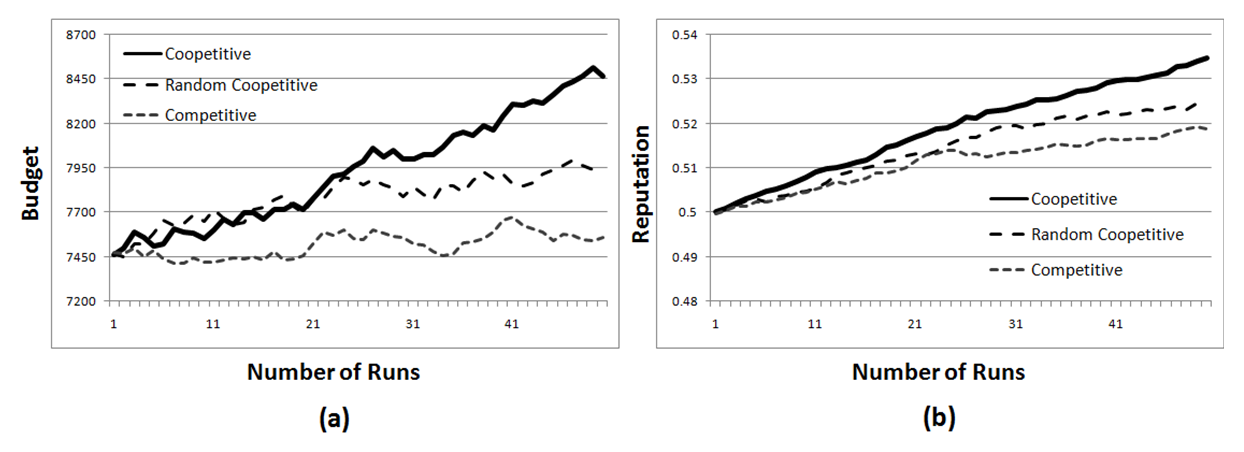
\includegraphics[scale=0.6]{graph1Final+.eps}
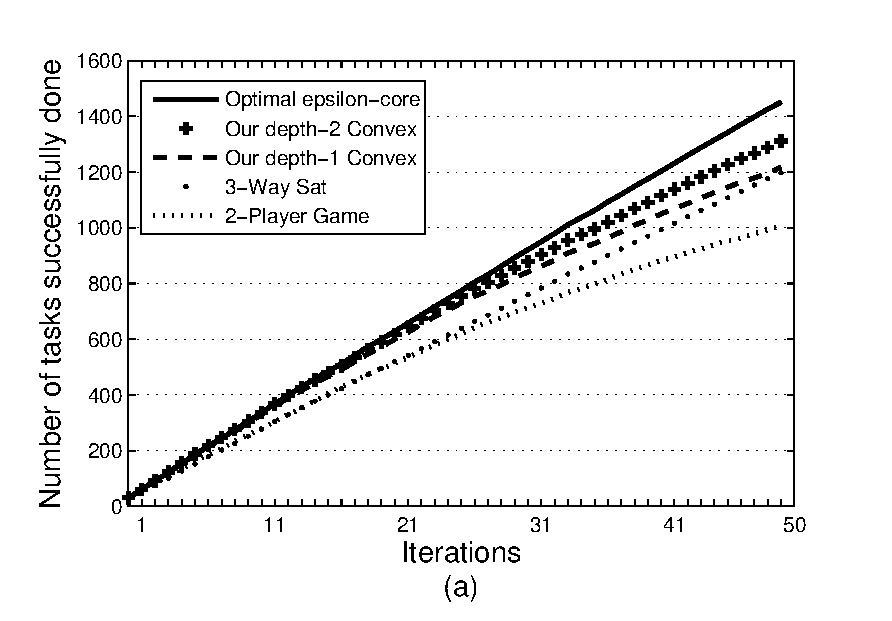
\includegraphics[width=2.8in]{task_done_opt.eps}
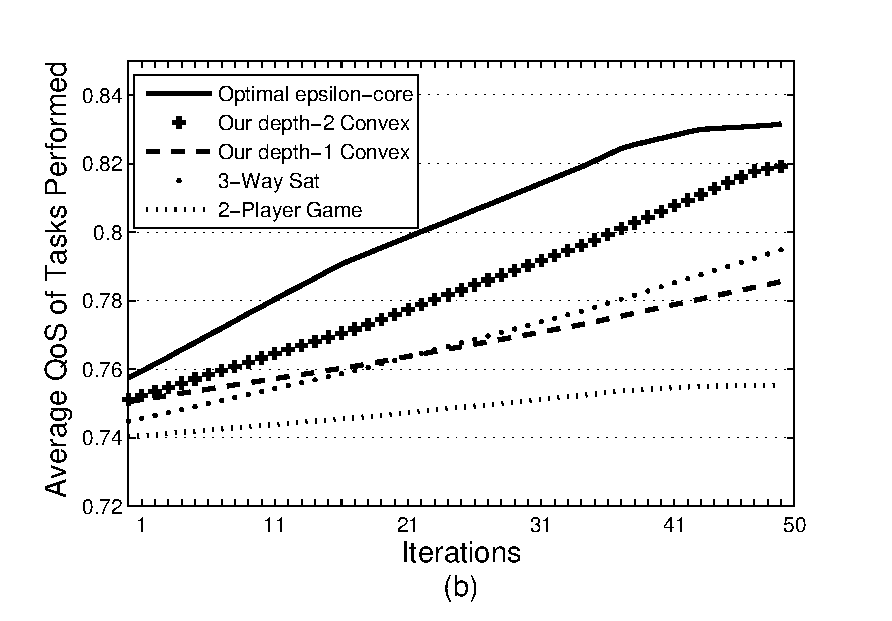
\includegraphics[width=2.8in]{task_qos_opt.eps}
\caption{Part (a): Cumulative number of requests successfully
done. Part (b): Average QoS of requests performed.}
\label{performanceall}
\end{figure*}

Figure \ref{performanceall} depicts the results of our methods:
\emph{Depth-1 Convex-Checker} and \emph{Depth-2 Convex-Checker},
and compares them with \emph{3-Way Satisfaction} (from
\cite{DBLP:conf/IEEEscc/LimTMB12}), and \emph{2 Player
Non-Cooperative} (from \cite{DBLP:conf/IEEEscc/KhosravifarABT11})
methods in \emph{one grand community with many web services}
scenario. The figure also depicts the results of the theoretical
\emph{optimal $\epsilon$-core} as benchmark.


For the \emph{optimal core} method, we have used the well known
\emph{$\epsilon$-core} method as the taxation method to relax the
core condition to help communities attract web services. We have
assigned $\epsilon$ to 15\% of total community worth, which means
$\epsilon = 0.15 \times v(C)$. This allows subsets of the
coalition to gain maximum 15\% of $v(C)$.
%In the \emph{optimal
%$\epsilon$-core} method, we capped the coalition size to 25 web
%services, since the method is computationally intractable as the
%number of web services increases. In fact, given the machine
%configuration we used in our experiments, the maximum number we
%could run for this method is 25, which is very realistic if we
%consider the real airlines coalitions (the three well known
%coalitions have respectively 28, 19, and 13 members). In the other
%methods, there were no cap on size of the community and we had
%communities of size 160 web services at some points, as discussed
%above.
In the experiments, our \emph{Depth-1 Convex-Checker} and
\emph{Depth-2 Convex-Checker} methods generate results instantly
(0.01ms in Java millisecond time unit granularity) in our machines
since their runtime with respect to the size of input (number of
web services) is $O(n)$ and $O(n^2)$ respectively. This shows that
the algorithms are efficient and the system is easily scalable. In
this scenario, our community receives 130 tasks from users on
average per iteration. These tasks are about flight booking and
are expected to be performed by the community. They are randomly
generated using a poisson distribution (having 130 as parameter).
Depending on community task queue and the assigned web services'
quality metrics the task will be performed with some qualities.
The community, after the task distribution process on each
iteration, will reevaluate QoS metrics of its members and can
check for new membership requests. Web services may join or leave
the community between iterations. The results show that our
\emph{depth-2 convex checker} method is performing better compared
to the other methods and its performance is close to the optimal
\emph{$\epsilon$-core} method. Our \emph{depth-1 convex checker}
and the \emph{3-Way Satisfaction} method, are also performing
well.

%
%\begin{figure*}%[!t]
%\centering
%%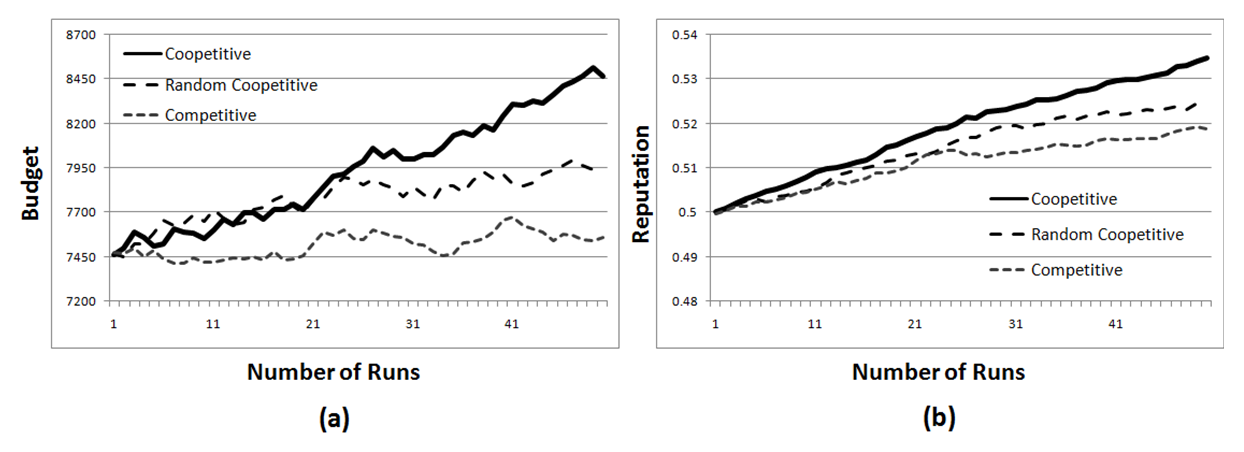
\includegraphics[scale=0.6]{graph1Final+.eps}
%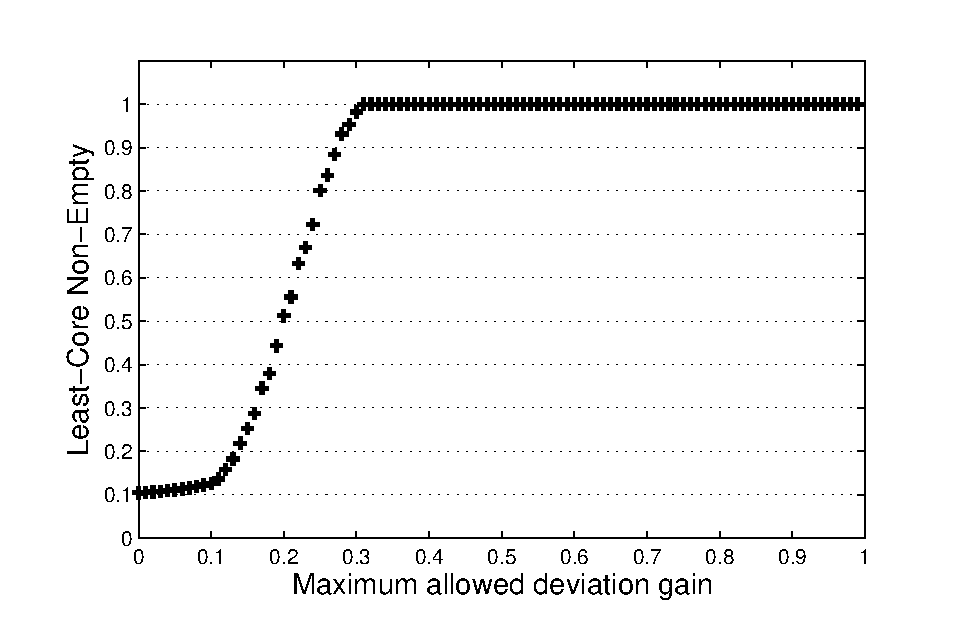
\includegraphics[width=3in]{least_core.eps}
%\caption{Analysis of \emph{$\epsilon$-core} set non-emptiness for
%different values of $\epsilon$} \label{f_leastcore}
%\end{figure*}
%
%As mentioned in Section \ref{s:preliminaries}, the concept of
%\emph{core}, assumes no coalition of players can gain anything by
%deviating, which is a fairly strong requirement, and that is why
%the notion of \emph{$\epsilon$-core} was introduced. Least-Core
%$e(G)$ of a game $G$ is the minimum amount of $\epsilon$ so that
%the core is not empty. We evaluated the non-emptiness of
%\emph{$\epsilon$-core} set using our valuation function and a set
%of web services from our coalitions.  The restriction on the
%number of web services per coalition for this particular method is
%justified because it is
%very complex for larger coalitions to verify whether
%\emph{$\epsilon$-core} set is empty or not. Also instead of
%considering $\epsilon$ amount of constant deviation in
%\emph{$\epsilon$-core} definition (Equation \ref{eq:core2}), we    %TODO FIX THIS
%similarly defined \emph{relative $\epsilon$-core} concept where no
%coalition would benefit more than \emph{$\epsilon \times v(C)$} by
%deviating. We vary $\epsilon$ so that it takes different values
%from $0$ to $1$ and observe the impact in terms of verifying the
%\emph{relative $\epsilon$-core} set non-emptiness. The results in
%Figure \ref{f_leastcore} illustrate that almost 10\% of our random
%web service coalitions have non-empty \emph{core} solution and
%\emph{$\epsilon$-core} solution is \emph{always} non-empty when we
%let agents gain only 30\% more of $v(C)$ by deviating.


\begin{figure*}%[!t]
\centering
%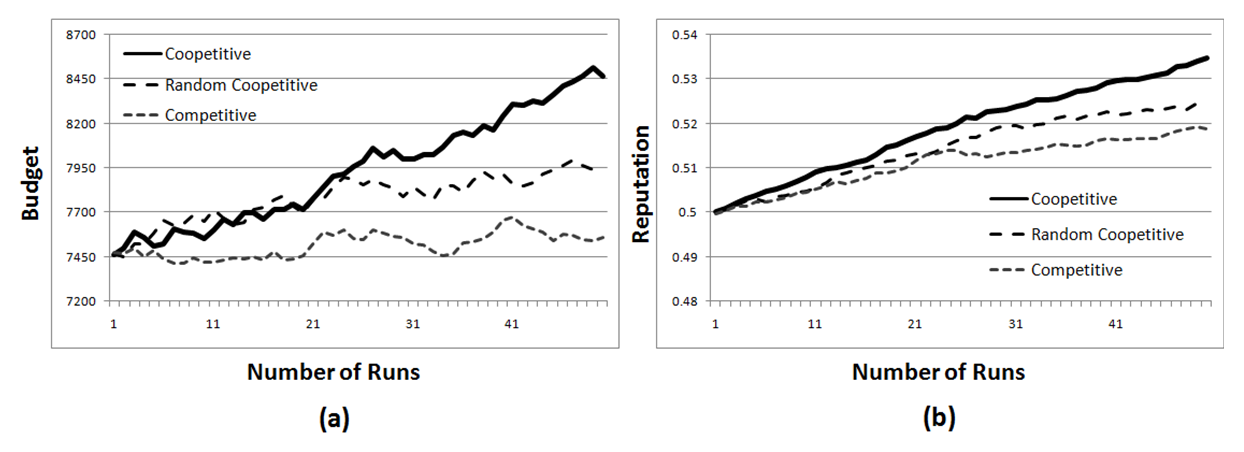
\includegraphics[scale=0.6]{graph1Final+.eps}
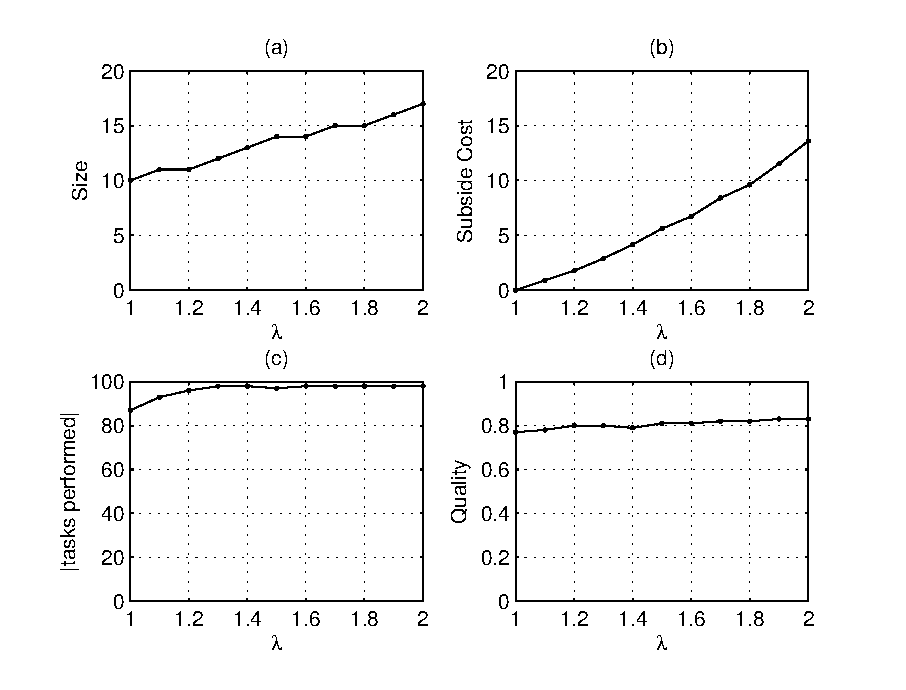
\includegraphics[width=3in]{taxtation.eps}
\caption{Analysis of community subsiding coefficient $\lambda$ on
average community size (a), cost (b), number of tasks performed
(c), and average quality of service of tasks performed (d).}
\label{f_taxtation}
\end{figure*}

As mentioned in Section \ref{s:tax}, a solution to help the
community stabilize is to subside the community by a relative
coefficient ($\lambda$) so the value of $\lambda v(C)$ is divided
among the community members. We have analyzed the effect of
subsiding and the cost it incurs to our web service communities.
Figure \ref{f_taxtation} shows the results. In this experiment, we
have set a community with input task rate $R_C$ of 100 and having
web services throughput rate $Th_{ws}$ values from a normal
distribution with average 10 tasks per iteration and standard
deviation 2. Part (a) shows the community size increases in a
linear fashion as ($\lambda$) increases. However, the cost (Part
(b)) is having a slight exponential growth rate since, not only
($\lambda$) increases, but also the size of the community is
increasing slowly. Therefore, subsiding can be costly for larger
number of $\lambda$ values. Part (c) depicts the number of tasks
done by the community per iteration. It is obvious that with
$\lambda$ value of 1.3, which is 30\% of the community valuation,
the number of tasks done almost reaches the input task rate cap of
100 tasks per iteration. The average quality of tasks also has a
slight increase since the community will be able to afford better
and more web services to join the community (Part (d)). These
results show the effectiveness of our subsiding method and its
impact on the QoS. In fact, using more than 30\% of the community
valuation as subsidy is not very effective and is costly to
perform.

\begin{figure*}%[!t]In the previous experiment, we considered the scenario where all
web services are stable, will not leave the group, and will
fulfill their promised QoS for a good period of time. However, in
real world scenarios of web services, this is not always the case.
This is the reason why the community coordinator would be interested in paying
web services in order to keep the group reliable from the end
user's point of view.
\centerline{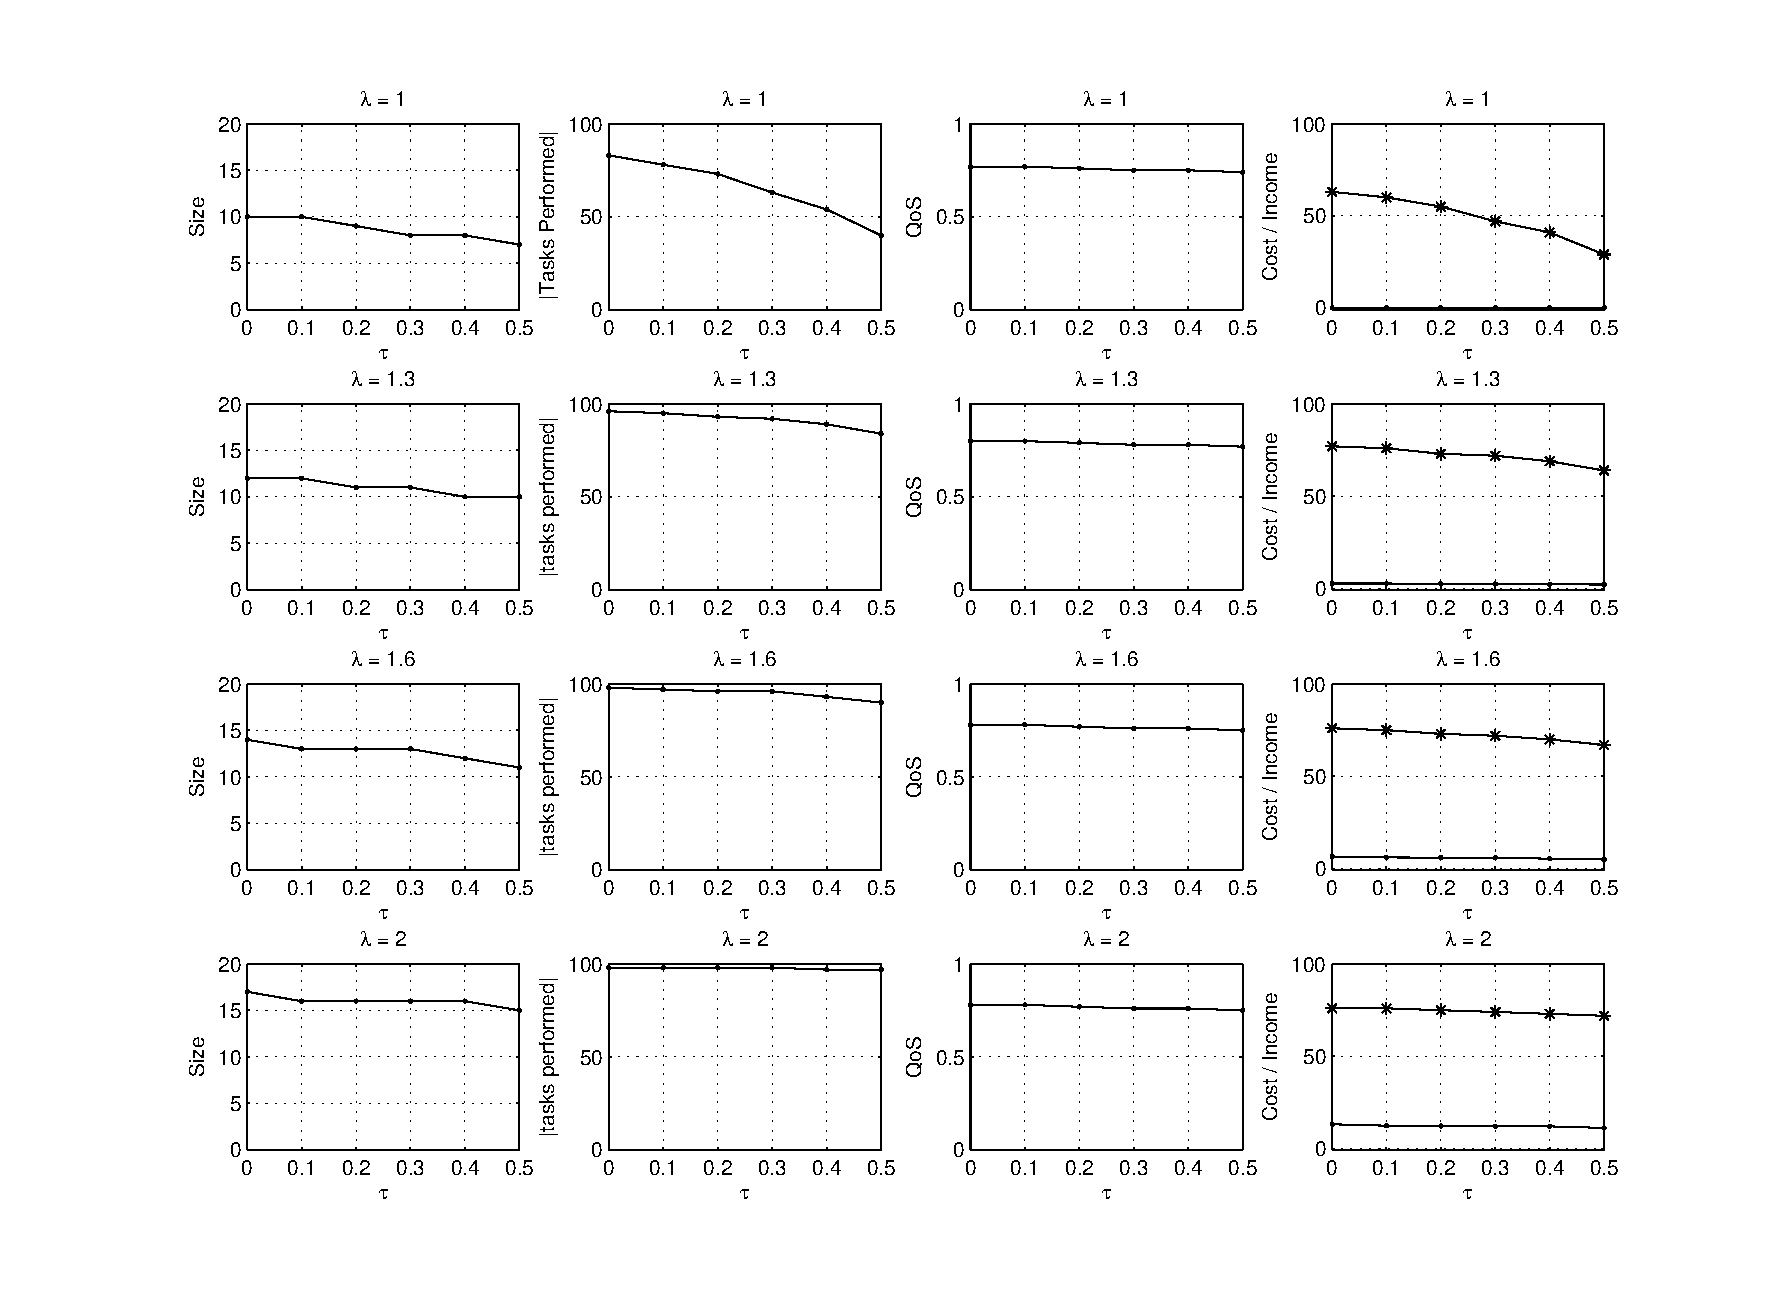
\includegraphics[width=6.8in]{tax_dyn.eps}}
\caption{Analysis of community subsiding coefficient $\lambda$
having web service different stability levels of $\tau$ on average
community size, number of tasks performed, average quality of
service, and average cost/income of communities.}
\label{fig_dynamic_taxtation}
\end{figure*}


In our next scenario, we have introduced the
new instability variable $\tau$ ranging from 0 to 1, 0 meaning web
services having no instability issues and will perform as they
claimed until the end of the experiment, and 1 meaning very
unstable web services, which will stop functioning on the first
iteration of the community distributing tasks. Figure
\ref{fig_dynamic_taxtation} illustrates the results of our
experiment having web services with average instability values of
0 to 0.5 and having relative subside value $\lambda$ of 1, 1.3,
1.6, and 2. The \emph{Cost/Income} charts on the right column show
that having subside value of 1.3 incurs the least cost and
increases the community income significantly. Subsiding values of
1.6 and 2 yield high cost to the community and only slightly
increase the community revenue. Moreover, the role of subsiding is
much more obvious when we have unstable web services. In scenarios
where web services are 100\% stable, the subsiding cost will
hardly be compensated by the community revenue.

\begin{figure*}%[!t]
\centering
%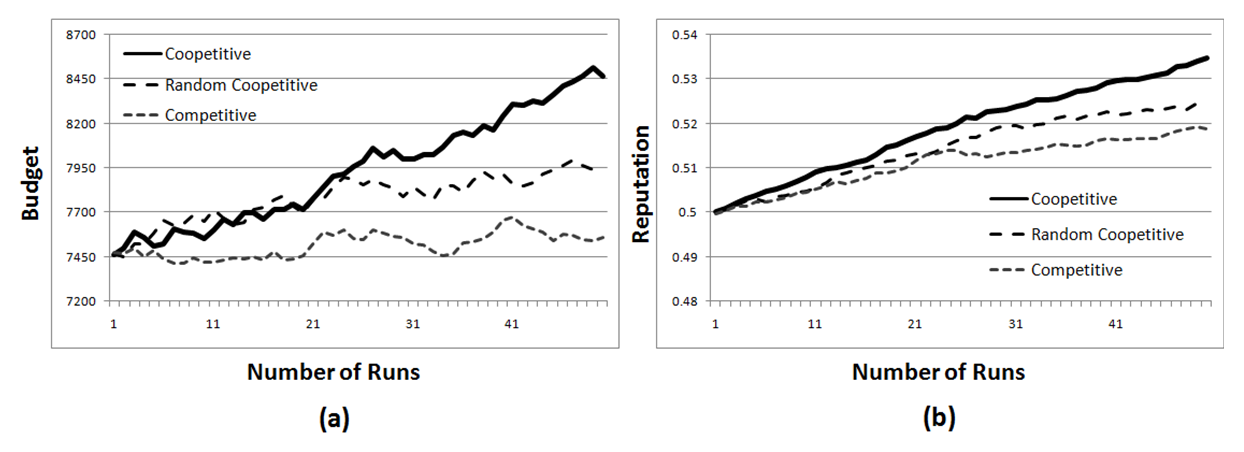
\includegraphics[scale=0.6]{graph1Final+.eps}
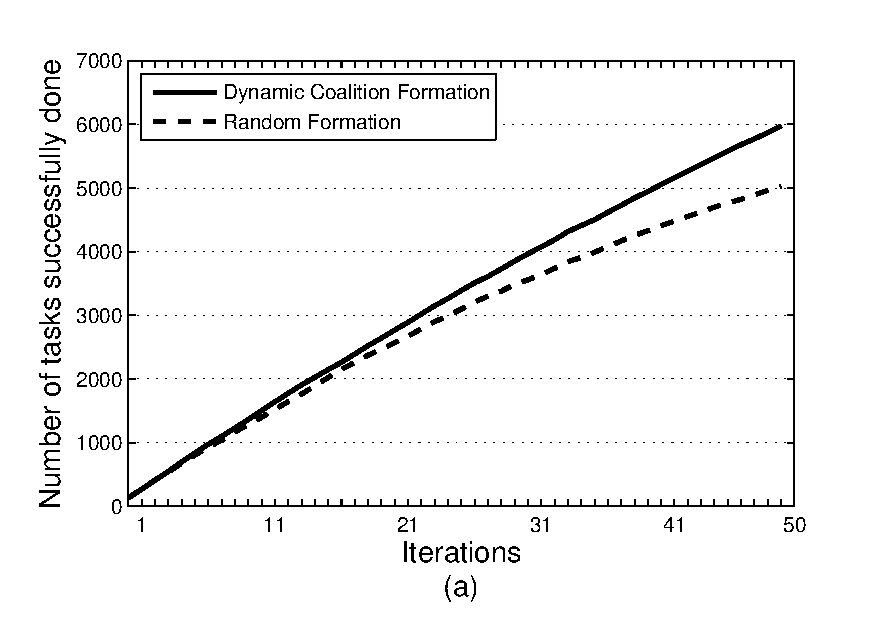
\includegraphics[width=2.8in]{s2_task_done.eps}
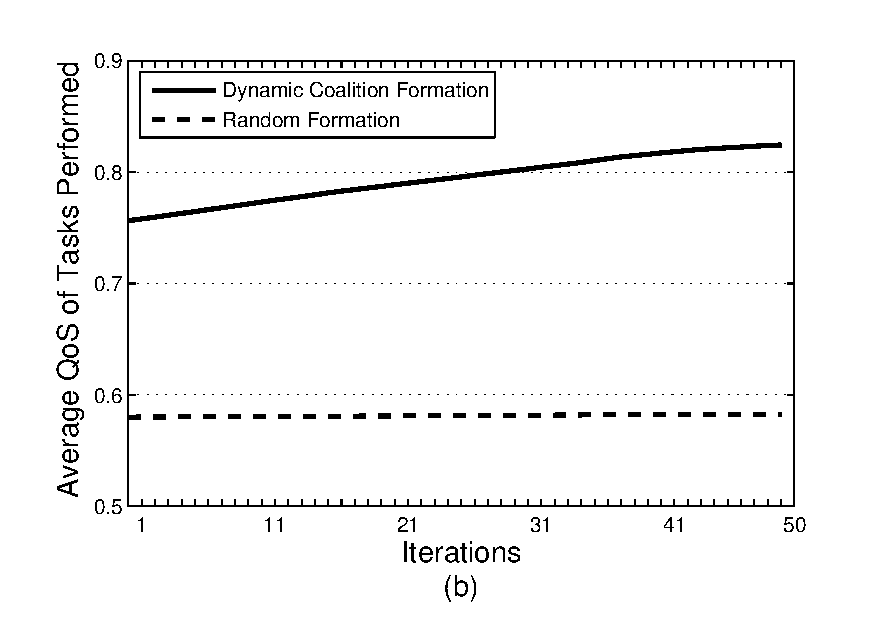
\includegraphics[width=2.8in]{s2_task_qos.eps}
\caption{Part (a): Cumulative number of tasks successfully done.
Part (b): Average QoS of tasks performed.} \label{performancemany}
\end{figure*}


In Figure \ref{performancemany}, we consider \emph{Web Services
and many Communities} scenario and we compare our dynamic
coalition formation solution with a method which ignores QoS
parameters and forms communities by allowing web services to join
only if they have enough requests for themselves. In other words,
web services can join a community when the request rate is less
than the throughput of all the member web services. We name this
method \emph{Random Formation} and use it as a benchmark for our
QoS-aware community formation process. In this scenario, each user
individually generates randomly between 0 to 10 number of tasks
per iteration, then the users target a community and direct their
requests to the chosen community. As the results illustrate, our
method forms better communities of web services improving
performance and satisfaction for both web services and
communities.

\begin{figure*}%[!t]
\centering
%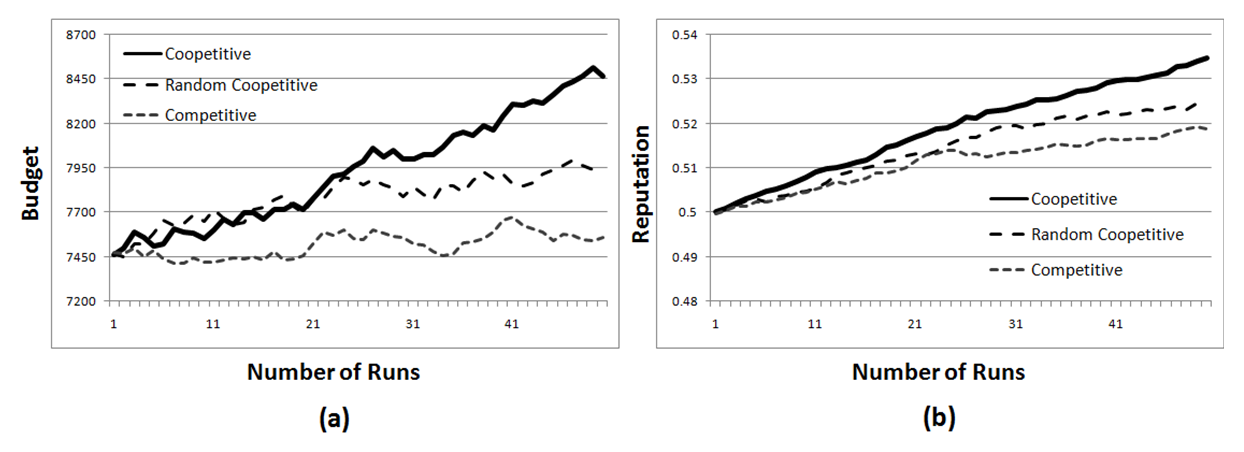
\includegraphics[scale=0.6]{graph1Final+.eps}
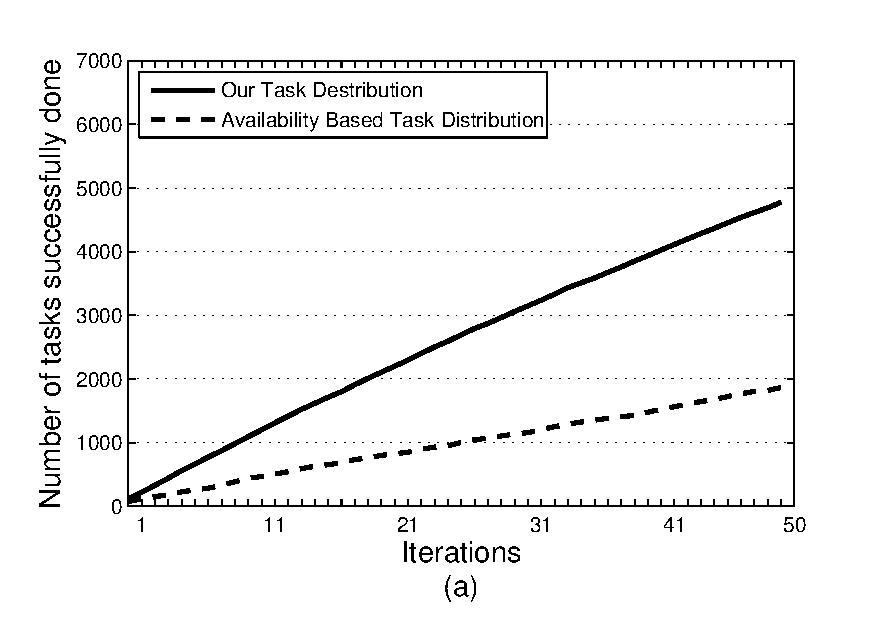
\includegraphics[width=1.9in]{avg_task_ws_done.eps}
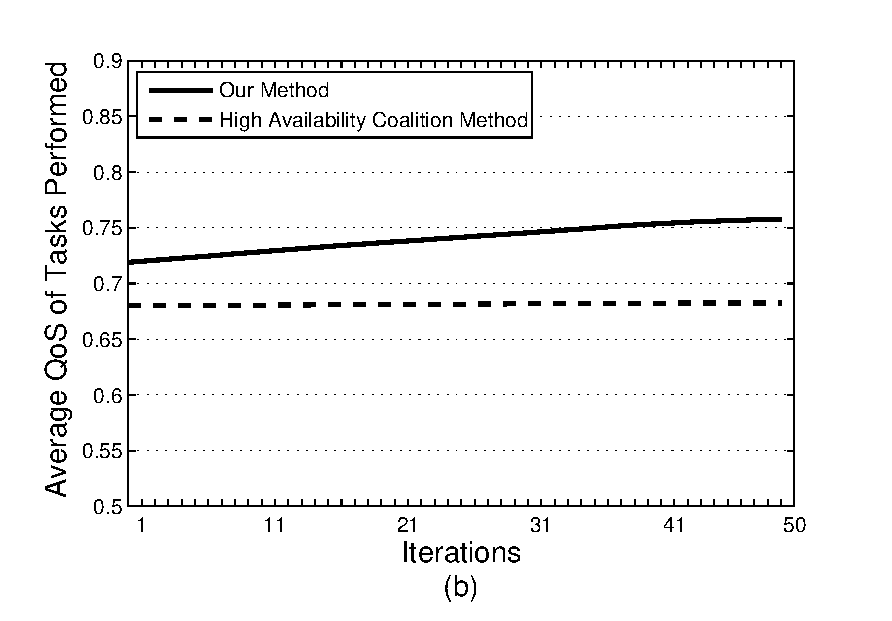
\includegraphics[width=1.9in]{avg_qos_ws_done.eps}
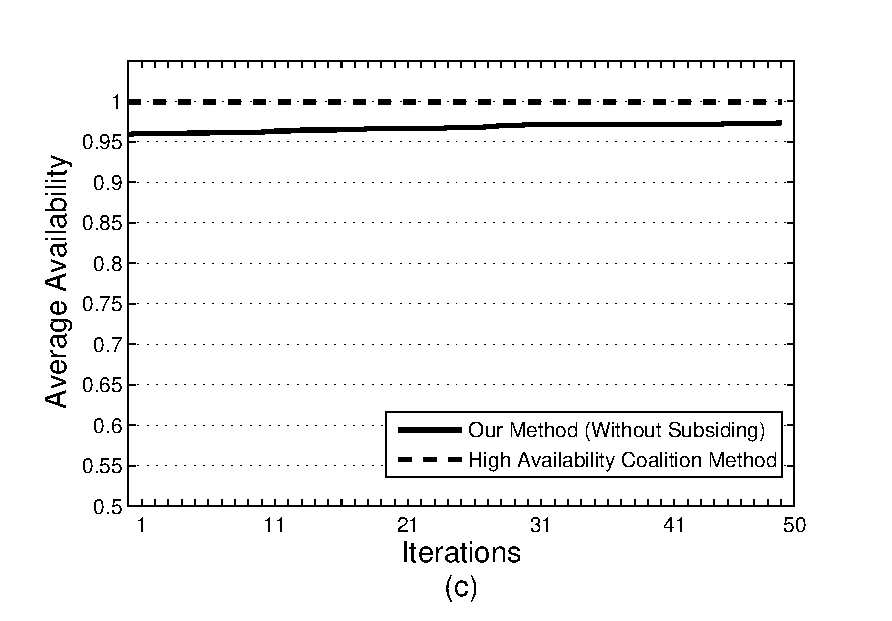
\includegraphics[width=1.9in]{avg_avail_ws_done.eps}
\caption{A comparison between our community model and the High
Availability Coalition model from \cite{10.1109/TSC.2012.12}. Part
(a): Cumulative number of tasks successfully done. Part (b):
Average QoS of tasks performed. Part (c): Average community
service availability} \label{fig_avail_method}
\end{figure*}

Finally, in our last experiment, we compare our model with the
solution proposed in \cite{10.1109/TSC.2012.12}, which we call
\emph{High Availability Coalition} model. In this method, the
community valuation function focuses on the community availability
as main consideration. The community formation model used in this
method is very different from ours, but we have been very careful
to make the experiment environment as fair and similar to ours as
possible. We limited our maximum community size to 5 in order to
have communities with almost the same size as in
\cite{10.1109/TSC.2012.12}. In the High Availability Coalition
model, the authors have used web services as backups rather than
active collaborative players, and those web services only get a
task when the first web service in an ordered chain fails to
perform that task. %However, with recent advancement in cloud and
%hardware infrastructures, availability is less of an issue for web
%services, and web services are highly available.
Part(a) of Figure \ref{fig_avail_method} shows that with our
method, the number of tasks successfully done is higher with a
rate of three times more than the High Availability Coalition
model thanks to the cooperative behavior of web services and the
task distribution process of our algorithm. This result shows that
using web services as backups, and not as real collaborative
players results in a considerable waste of web services capability
since services have very low chance of getting jobs and its the
primary web service (the first in the coordination chain) which
does most of the work. As shown in Part (b), the average quality
of service of tasks performed using our solution is also higher
since our method considers all quality of service metrics used. Part(c) shows the availability of
communities from the end user's point of view. The High
Availability Coalition model has almost 100\% uptime since web
services are used as backups, so the chance of job failing is
getting reduced significantly as community members increase. In
our method, we have more chance of failure for each web service.
However, with some subsidies and by hiring a few more web
services, the chance of failure of web services in our communities
can be lowered.

\subsection*{Coopetitive behaviour of services within communities}\label{sb:resutlscoop}

In this section, the objective is to investigate the effectiveness of the proposed strategic system in section \ref{s:coop}.
We start our discussions with cumulative budget comparison
regarding different communities within which services follow
different reasoning techniques. Figure \ref{Graph1} part (a)
illustrates three graphs for three different communities. Each
community hosts services that follow different reasoning
techniques: (1) a community that follows the interactive reasoning
techniques presented in this report (referred to as coopetitive);
(2) a community that follows a stochastic reasoning technique so
decisions about selecting competitive or cooperative strategies
are totally random (referred to as random coopetitive); and (3) a
competitive community where all services follow the competitive
strategy (referred to as competitive).
%The proposed model's
%reasoning mechanism allows services to make decisions that
%maximize their utilities, so that if the service cannot compete,
%the procedure would suggest to collaborate, which is better than
%competing and failing to obtain the task. In this case, the service stays idle but
%still pays the community membership fee, which means losing
%utility. The developed strategic decision making mechanism leads
%some service agents to follow cooperative strategies that overall
%maintain an optimal community budget. In the same figure, we
%observe the cumulative budget of a community where services follow
%random interacting strategies. The outcome is clearly lower
%because services at each run randomly decide over their acting
%strategies. This potentially influences the community budget
%because a low quality service if randomly selects to follow the
%competitive strategy, it will fail to perform a task with high QoS
%requirements.


The results illustrated in Figure \ref{Graph1} part (a)  verify
the importance of the strategic decision making procedure to
logically decide over the possible competitive and cooperative
choices. Figure \ref{Graph1} part (b) illustrates communities
average reputation of involved services. The graphs represent the
influence of the rewards that the master agent uses to encourage
highly capable services to compete for a task. As for the
cumulative budget, we observe that the coopetitive community
outperforms the random coopetitive and competitive communities in
terms of average reputation. The proposed model's average
reputation increases because services follow optimal strategies
where they can perform better so obtain higher rewards. For the
same reasons as for the cumulative budget, the average reputation
of the random coopetitive community
outperforms the one of the competitive community. %The idea is to balance web
%services' strategies to maintain optimal community budget.


\begin{figure}%[h]
%\centering
%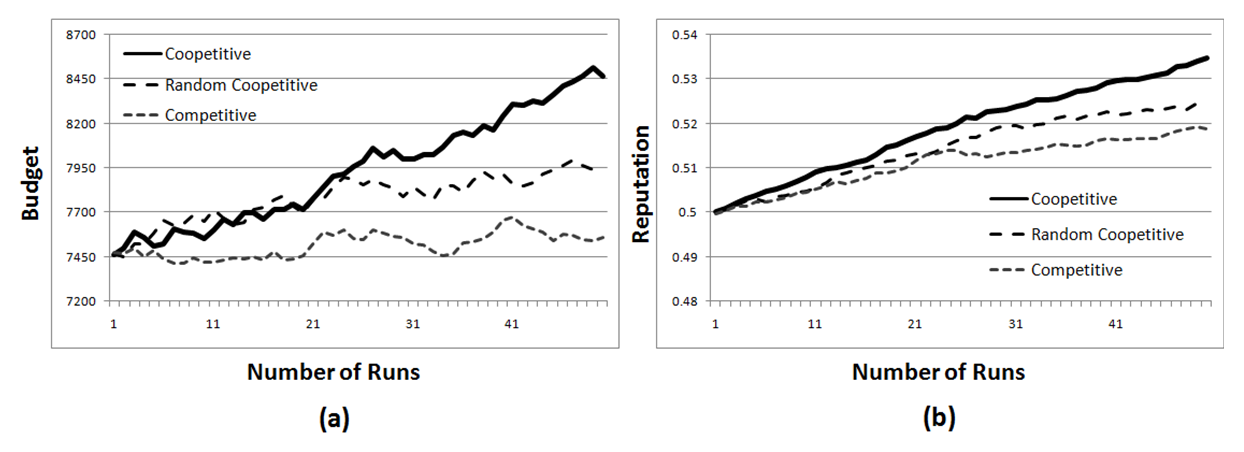
\includegraphics[scale=0.6]{graph1Final+.eps}
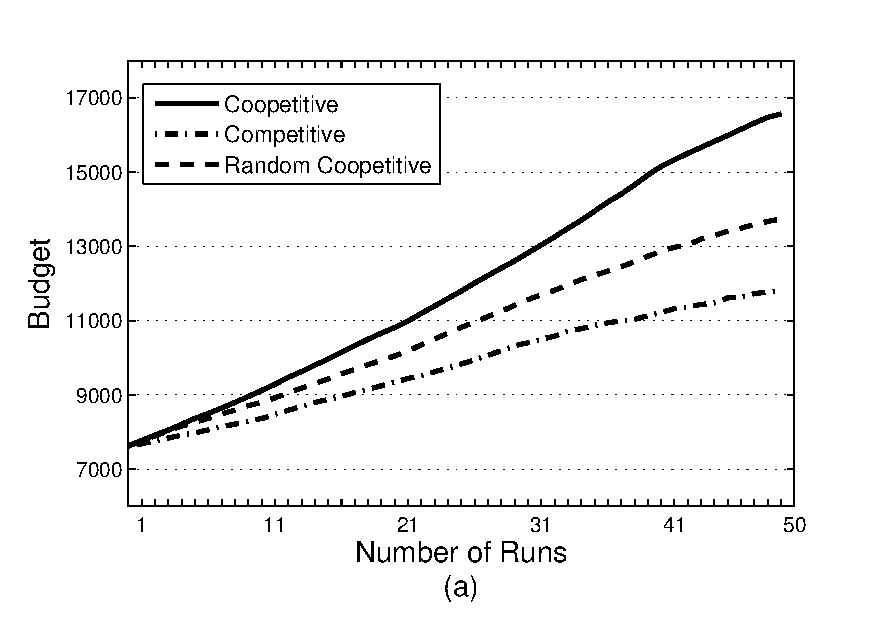
\includegraphics[scale=0.47]{graphbgtmed.eps}
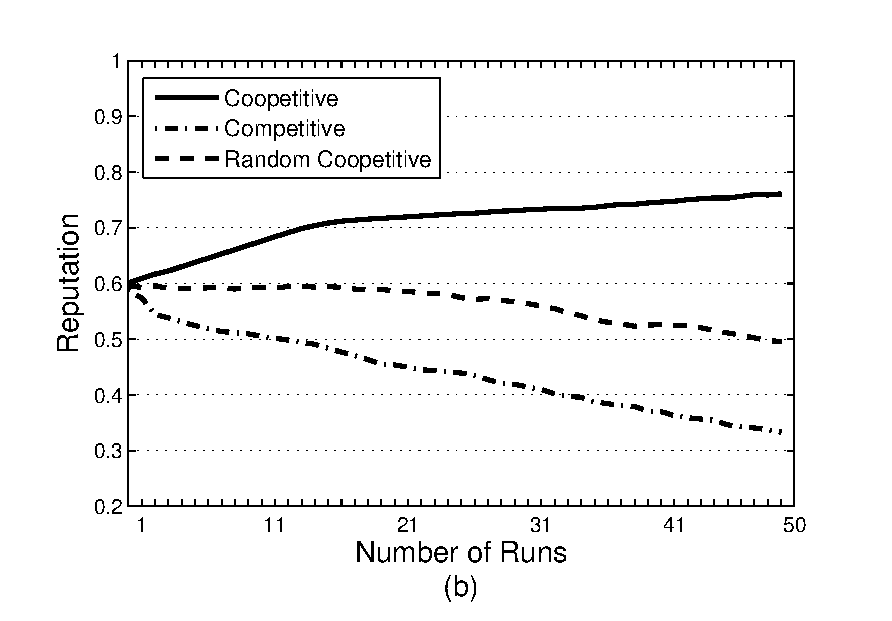
\includegraphics[scale=0.47]{graphrep.eps}
\caption{Part (a): Cumulative community budget comparison. Part
(b): Average community reputation comparison over different
strategic decisions.} \label{Graph1}
\end{figure}



 %Figure \ref{Graph2} part (a) illustrates the reputation of the proposed $Coopetitive$ community where
 %we highlight the range of reputation change in the community. The vertical lines denote the range of %reputation that is associated with the master web service. The rewards and penalties applied to %different
% web services show that the master web service over runs extends the reputation range and takes %control of the whole community. In the developed model, web services are encouraged to choose
 %optimal strategies. This is maintained over growth factor comparison of the $Coopetitive$ web %services.


In our model, services are managed by selfish agents in the sense
they try to maximize their own utilities. We analyze how their
strategies affect the social welfare, and from user's and
community's point of view how good the tasks are being performed.
This directly impacts user's satisfaction and community's
reputation in general. The Higher quality and quantity of tasks
performed leads to higher user's satisfaction for the community
which results in better reputation for the community. The results
in Figure \ref{graph_task} show the quality and quantity of tasks
being done successfully in three communities adopting the three
different aforementioned strategy decision algorithms. As clearly confirmed by the simulation, the coopetitive community
outperforms the stochastic and compete communities.

\begin{figure}[h]
\centering
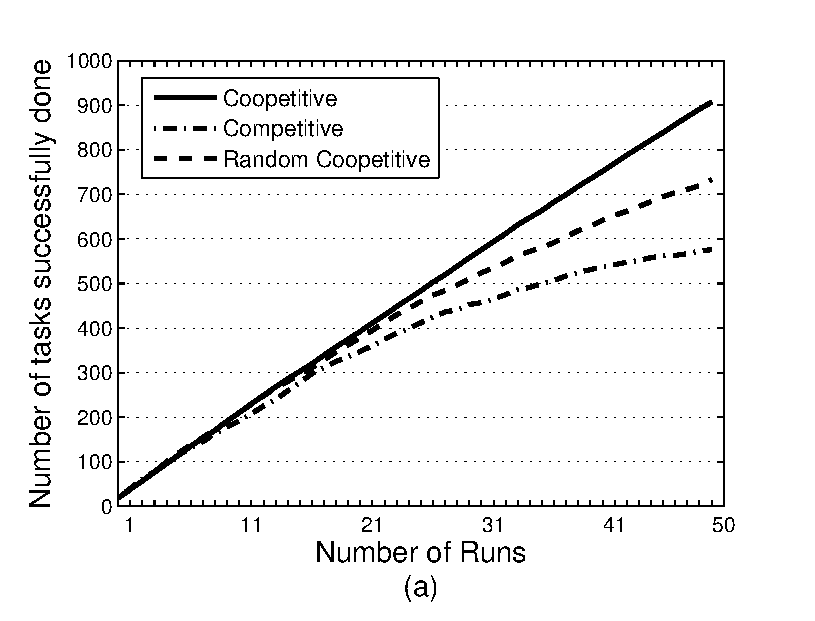
\includegraphics[scale=0.35]{graphtaskdone.eps}
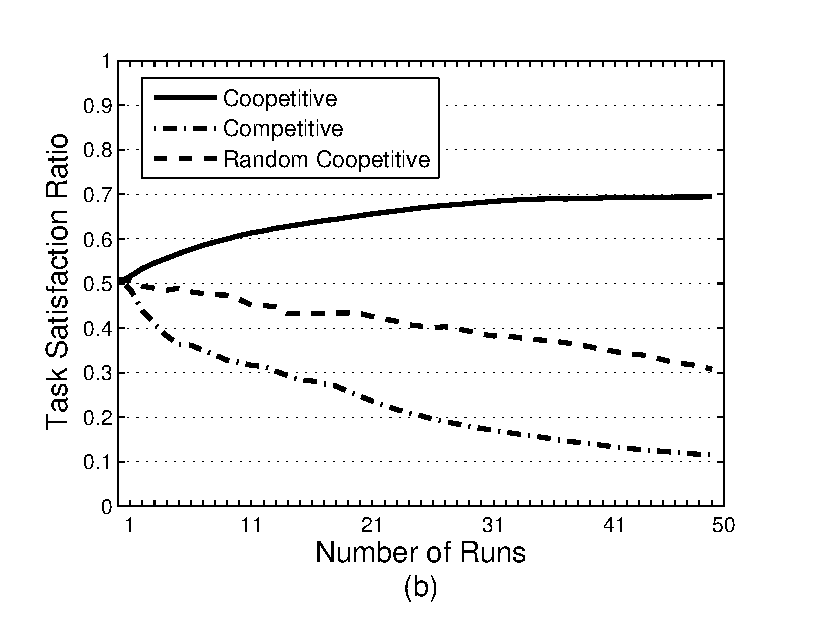
\includegraphics[scale=0.35]{graphtasksatisfaction.eps}
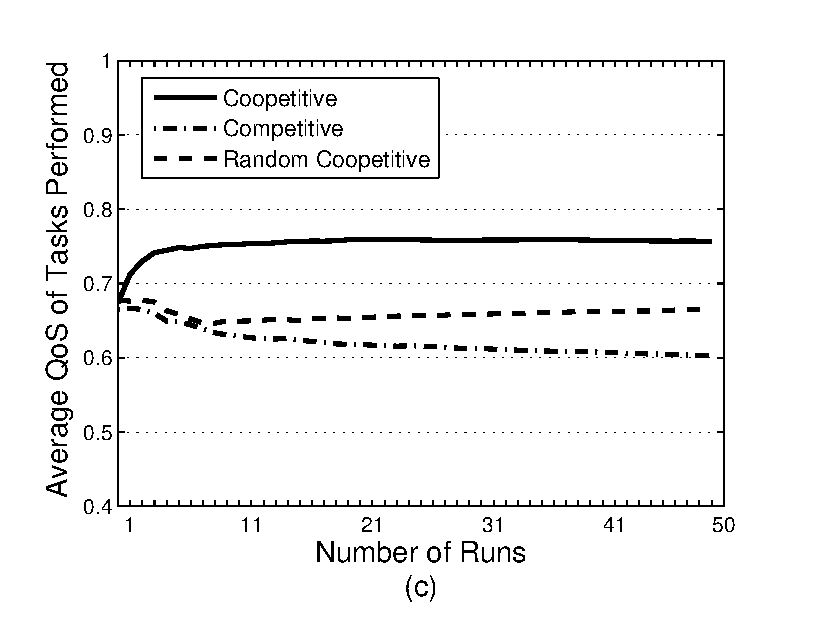
\includegraphics[scale=0.35]{graphavgqostask.eps}
\caption{Overall performance from community's point of view. Part
(a) Total number of tasks successfully done. Part (b) Ratio of
tasks satisfied with required QoS. Part (c) Average QoS of
performed tasks.} \label{graph_task}
\end{figure}


%\setcounter{chapter}{3}

\chapter{Conclusion and Future Work}

\section{Conclusion}\label{sec:conclusion}
In this paper, we proposed a new set of uncertainty measures for the agents in argumentation-based negotiation dialogues from an
external agent's point of view. Specifically, we introduced two types of uncertainty measures: 1) Type I, the uncertainty index of
playing the right move at each dialogue step; and 2) Type II, the uncertainty degree of the agent that the move will be accepted by
the addressee.
For uncertainty Type I, we used Shannon entropy to assess the agents' uncertainty/certainty about their moves in the negotiation
dialogues. We supposed that an external agent is monitoring the dialogue, and he wants to evaluate this dialogue in terms of the
agent's uncertainty/certainty about selecting the right move at each step. In fact, at each step, the agent is supposed to have
different choices, each choice is associated with a probability of being the right one, %which represents the risk of failure for this move to be accepted by the addressee.
this probability reflects the importance of information included in that move, where the higher the probability is, the
more certain the agent becomes (lower uncertainty). So we analyzed the fact that negotiating agents are rational, and they always
try to perform the actions that will result in the optimal outcome for themselves. We used Shannon entropy to measure: i) the
uncertainty/certainty index and the weighted uncertainty/certainty index of the agent that he is playing the right move at each
step during the dialogue; and ii) the uncertainty/certainty index and the weighted uncertainty/certainty index of both agents
participating in the dialogue about the whole dialogue. This was done in two different ways. The first is by taking the average of
the uncertainty index of all moves, and the second is by determining all possible dialogues and applying the general formula of Shannon entropy.

For uncertainty Type II, we formalized the probability association to the arguments and the uncertainty that the move will be
accepted by the addressee. In this context, we introduced a new classification of arguments based on the notion of risk of failure
and showed that this classification is compatible with the probability that the moves supported by those arguments will be
accepted by the address. An important result of this paper is that the selection and probability ordering mechanisms of arguments
are tractable as they can be performed in polynomial time if arguments are represented in propositional definite Horn logic.

In our proposed measures, the move with the higher certainty (lower uncertainty) index is considered as the best move. We analyzed
the fact that negotiating agents are rational, and they always try to perform the actions that will result in the optimal outcome
for themselves. We started our work with measuring the uncertainty/certainty index of each move at each dialogue step, and in order
to distinguish between two moves with the same certainty index, we assigned weight to each move, which reflects the importance of the
move. Then, we proceeded to the whole dialogue and we measured the uncertainty/certainty index for the dialogue in two different ways,
and we proved that the two ways give the same result. Also, assigning weight to the moves allowed us to compare two different dialogues.
We believe that such measures are very significant and helpful in evaluating the dialogue and the agent's strategies, especially when
they are making a decision and selecting the best moves to achieve an agreement (if one exists) in a timely manner.



\section{Future Work}\label{sec:future}
In this paper, we mainly focused on the classical (i.e., precise) probability theory, particularly the classical Shannonian
information theory to measure the uncertainty. As pointed out in \cite{Harmanec1999}, there are other approaches of measuring
uncertainty in the theories of imprecise probabilities, particularly the Dempster-Shafer theory (also known as the theory
of belief functions) \cite{Shafer76} and the possibility theory \cite{Dubois2001}. As future work, we will study key measurements
in these two theories such as \emph{nonspecificity}, \emph{confusion}, \emph{dissonance}, \emph{discord}, and \emph{strife}, and
we will adapt, define and integrate them in our framework. Combining and aggregating those measurements to finally measure the
total uncertainty will be investigated as well. The requirements of those new metrics as reported in \cite{Harmanec1999} will be
analyzed. Those requirements are: 1) generalization, meaning that the new uncertainty measures should generalize the uncertainty
measures already established in the classical probability theory; 2) subadditivity, meaning that when the problem is broken into
two orthogonal subproblems, the uncertainty of the original problem should be less than or equal to the sum of uncertainties of the
subproblems; and 3) additivity, meaning that under the assumption of no interaction and no dependency between the subproblems, the
uncertainty of the original problem is equal to the sum of uncertainties of the subproblems.

Another plan for future work is to extend the proposed metrics for other dialogue game types such as persuasion, deliberation,
inquiry and information seeking. We also plan to analyze argumentation-based dialogues to evaluate agent strategies and
analyze them from the optimization perspective. Analyzing the computational complexity of such optimization problems is another
direction for future work. Finally, we plan to analyze multi-party dialogues to which many agents can participate. Extending the
proposed metrics to this type of dialogues is not straightforward. For example, defining the rules of a multi-party negotiation is
much more complicated than two-party dialogues. In fact, multi-party dialogues cannot be simply reduced to many two-party dialogues.









\setcounter{chapter}{3}
\chapter{Conclusion and Future Work}
In this chapter, we describe the phases of our plan for exploring the research challenges and investigating the research issues identified in Chapter 4. This chapter also includes research methodology and future publication plan.

\section {Conclusion}

In this report, we proposed a cooperative game theory-based model
for the aggregation of web services within communities. The goal
of our services is to maximize efficiency by collaborating and
forming stable coalitions. Our method considers stability and
fairness for all web services within a community and offers an
applicable mechanism for membership requests and selection of web
services. The ultimate goal is to increase revenue by improving
user satisfaction, which comes from the ability to perform more
tasks with high quality. Simulation results show that our,
polynomial in complexity, approximation algorithms provide web
services and community owners with applicable and near-optimal
decision making mechanisms.

%As future work, we would like to perform more analytical and
%theoretical analysis on the convexity condition and also minimal $\epsilon$ values in \emph{$\epsilon$-core} solution concepts based on the
%characteristic function in web service applications. From web service perspective, the
%work can be extended to consider web service compositions where a
%group of web services having different set of skills cooperate to
%perform composite tasks. Also bargaining theory from cooperating
%game theory concepts can be used to help web services resolve the
%instability and unfairness issues by side payments.

\section {Future Plan and Timeline}

\indent The future goals in this PhD research work mainly consists of:

\begin{itemize}
\item Analysing other cooperative solution concepts such as Kernel and Nucleolus where payoff division is guaranteed to exist but may have optimal results.
\item Applying Weighted Voting Games (WCG) type of valuation function in our scenarios, Developing a multiple weighted algorithm to find best coalition structures satisfying different weights on each community.
\item Implementing Q-learning and reinforcement learning technique and also a tic-tac-toe based repeated game technique for individual Web Service decision making process, in long term and repeated game scenarios.
\item Developing an approximation algorithm for shapely value payoff distribution vector in community of service setting.    
\item Developing a community membership algorithm technique for our agents in "incomplete information" settings.
\item Developing an open source, Java based Tool, with UI for solving Core and Shapely solution concepts based on different input valuation functions.
\end{itemize}


    \begin{figure}
                \begin{center}
%                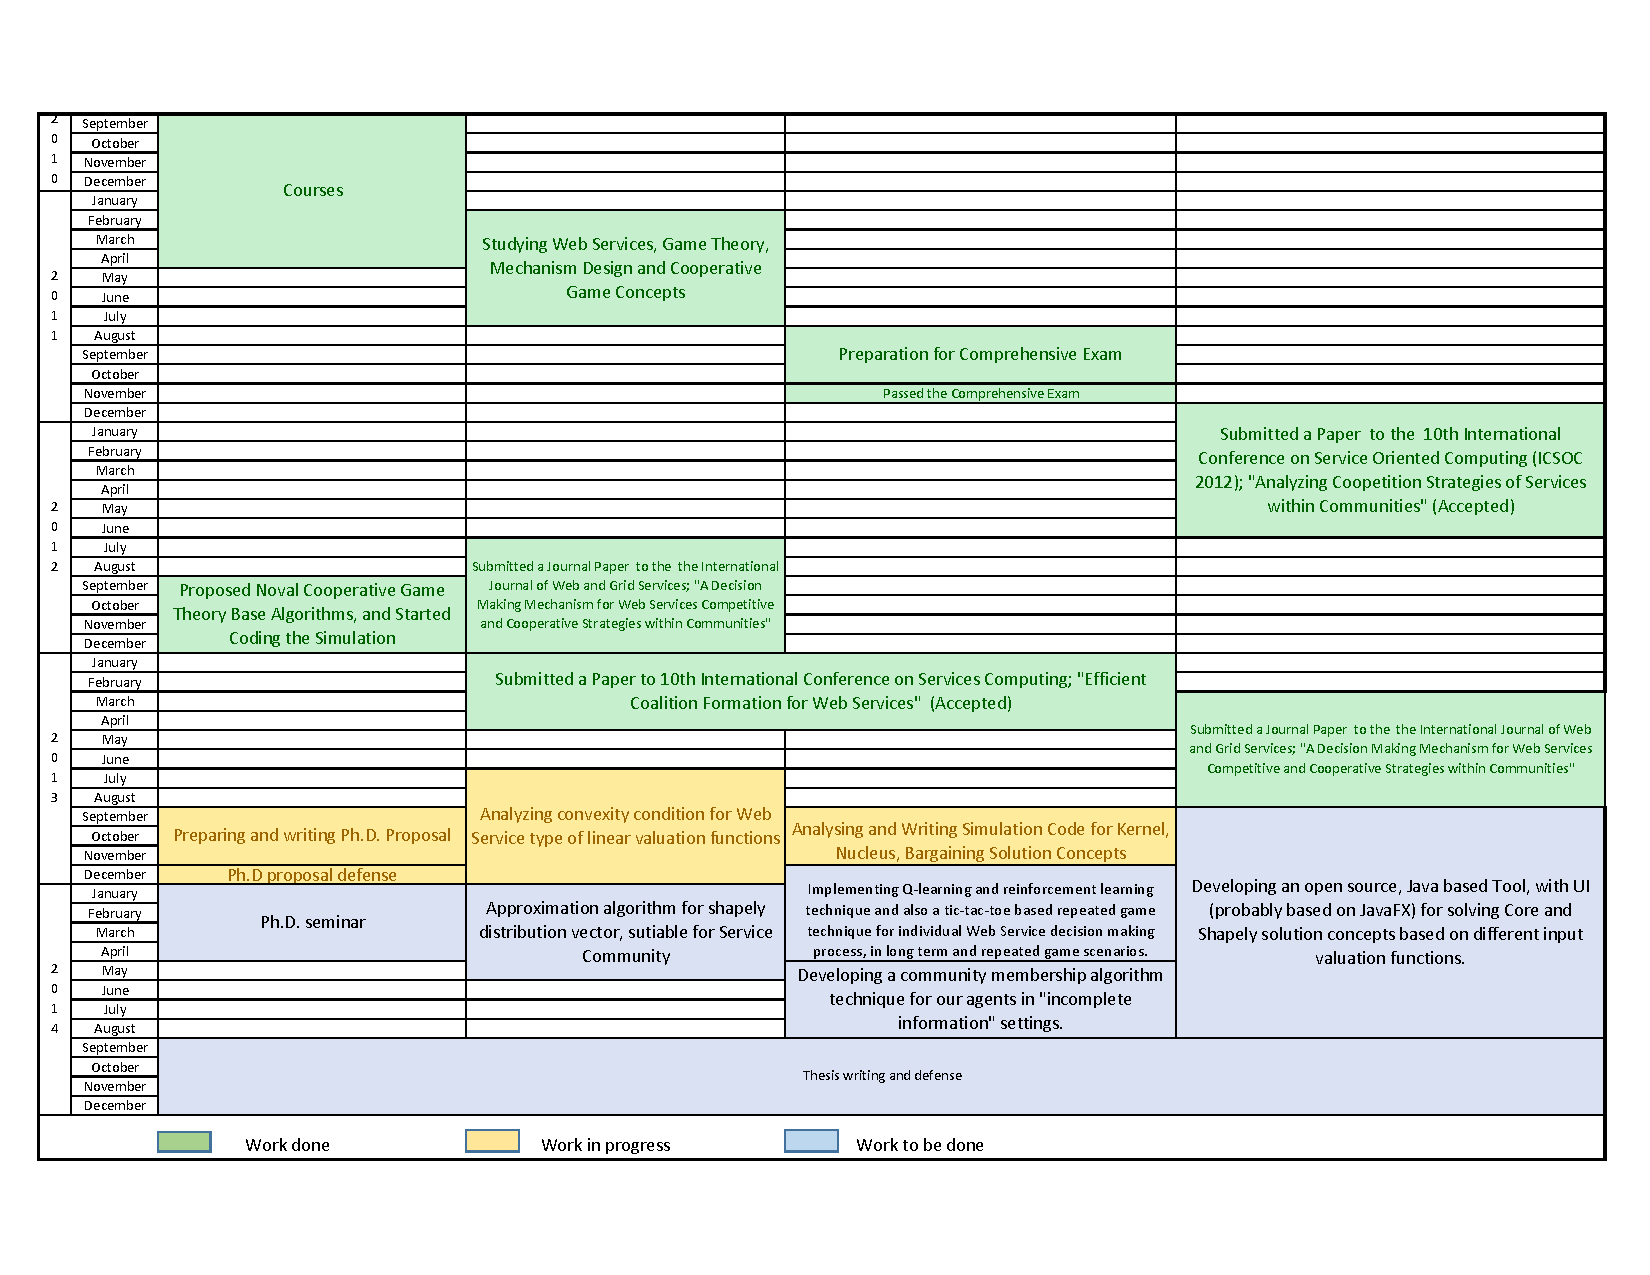
\includegraphics[width=16cm, height=22cm]{timeline/timetable.pdf}\label{Timetable}
                \includegraphics[width=16cm]{Figures/fw.eps}\label{Timetable}
                \caption{Research milestones and time line}
                \end{center}
    \end{figure}   
%\include{chapter6}
%\include{chapter7}
%\bibliography{omar}
%\bibliography{NNBbibliography}

%\bibliography{NNBbibliography,IEEEabrv,WDM_Networks,lp,telecom,pCycles,WDM_protection}
%\addcontentsline{toc}{chapter}{Bibliography}
%\chapter*{Appendix}
%\input{appendix}
%\addcontentsline{toc}{chapter}{Appendix}
%\appendix
%\include{appendix_notation}
%\chapter*{Vita}//uncomment
%\input{vita.tex}

%******************** START Bibliography*******************************************
\newpage
\pagestyle{plain}
%The following adds references to the table of contents
\addcontentsline{toc}{chapter}{Bibliography}
%\addchapter*{Bibliography}
%Give the name of your bibtex database
\bibliography{ehsan}
\bibliographystyle{plain}
%\clearpage

%\bibliographystyle{unsrt}

%******************** END Bibliography*********************************************

\end{document}
